% Options for packages loaded elsewhere
\PassOptionsToPackage{unicode}{hyperref}
\PassOptionsToPackage{hyphens}{url}
%
\documentclass[
  11pt,
]{article}
\usepackage{amsmath,amssymb}
\usepackage{lmodern}
\usepackage{ifxetex,ifluatex}
\ifnum 0\ifxetex 1\fi\ifluatex 1\fi=0 % if pdftex
  \usepackage[T1]{fontenc}
  \usepackage[utf8]{inputenc}
  \usepackage{textcomp} % provide euro and other symbols
\else % if luatex or xetex
  \usepackage{unicode-math}
  \defaultfontfeatures{Scale=MatchLowercase}
  \defaultfontfeatures[\rmfamily]{Ligatures=TeX,Scale=1}
\fi
% Use upquote if available, for straight quotes in verbatim environments
\IfFileExists{upquote.sty}{\usepackage{upquote}}{}
\IfFileExists{microtype.sty}{% use microtype if available
  \usepackage[]{microtype}
  \UseMicrotypeSet[protrusion]{basicmath} % disable protrusion for tt fonts
}{}
\makeatletter
\@ifundefined{KOMAClassName}{% if non-KOMA class
  \IfFileExists{parskip.sty}{%
    \usepackage{parskip}
  }{% else
    \setlength{\parindent}{0pt}
    \setlength{\parskip}{6pt plus 2pt minus 1pt}}
}{% if KOMA class
  \KOMAoptions{parskip=half}}
\makeatother
\usepackage{xcolor}
\IfFileExists{xurl.sty}{\usepackage{xurl}}{} % add URL line breaks if available
\IfFileExists{bookmark.sty}{\usepackage{bookmark}}{\usepackage{hyperref}}
\hypersetup{
  hidelinks,
  pdfcreator={LaTeX via pandoc}}
\urlstyle{same} % disable monospaced font for URLs
\usepackage[margin=1in]{geometry}
\usepackage{longtable,booktabs,array}
\usepackage{calc} % for calculating minipage widths
% Correct order of tables after \paragraph or \subparagraph
\usepackage{etoolbox}
\makeatletter
\patchcmd\longtable{\par}{\if@noskipsec\mbox{}\fi\par}{}{}
\makeatother
% Allow footnotes in longtable head/foot
\IfFileExists{footnotehyper.sty}{\usepackage{footnotehyper}}{\usepackage{footnote}}
\makesavenoteenv{longtable}
\usepackage{graphicx}
\makeatletter
\def\maxwidth{\ifdim\Gin@nat@width>\linewidth\linewidth\else\Gin@nat@width\fi}
\def\maxheight{\ifdim\Gin@nat@height>\textheight\textheight\else\Gin@nat@height\fi}
\makeatother
% Scale images if necessary, so that they will not overflow the page
% margins by default, and it is still possible to overwrite the defaults
% using explicit options in \includegraphics[width, height, ...]{}
\setkeys{Gin}{width=\maxwidth,height=\maxheight,keepaspectratio}
% Set default figure placement to htbp
\makeatletter
\def\fps@figure{htbp}
\makeatother
\setlength{\emergencystretch}{3em} % prevent overfull lines
\providecommand{\tightlist}{%
  \setlength{\itemsep}{0pt}\setlength{\parskip}{0pt}}
\setcounter{secnumdepth}{-\maxdimen} % remove section numbering
\usepackage{subfig} \usepackage{fancyhdr} \thispagestyle{empty} \usepackage{titling} \pretitle{\centering \vspace*{-1cm}\hspace*{-1cm}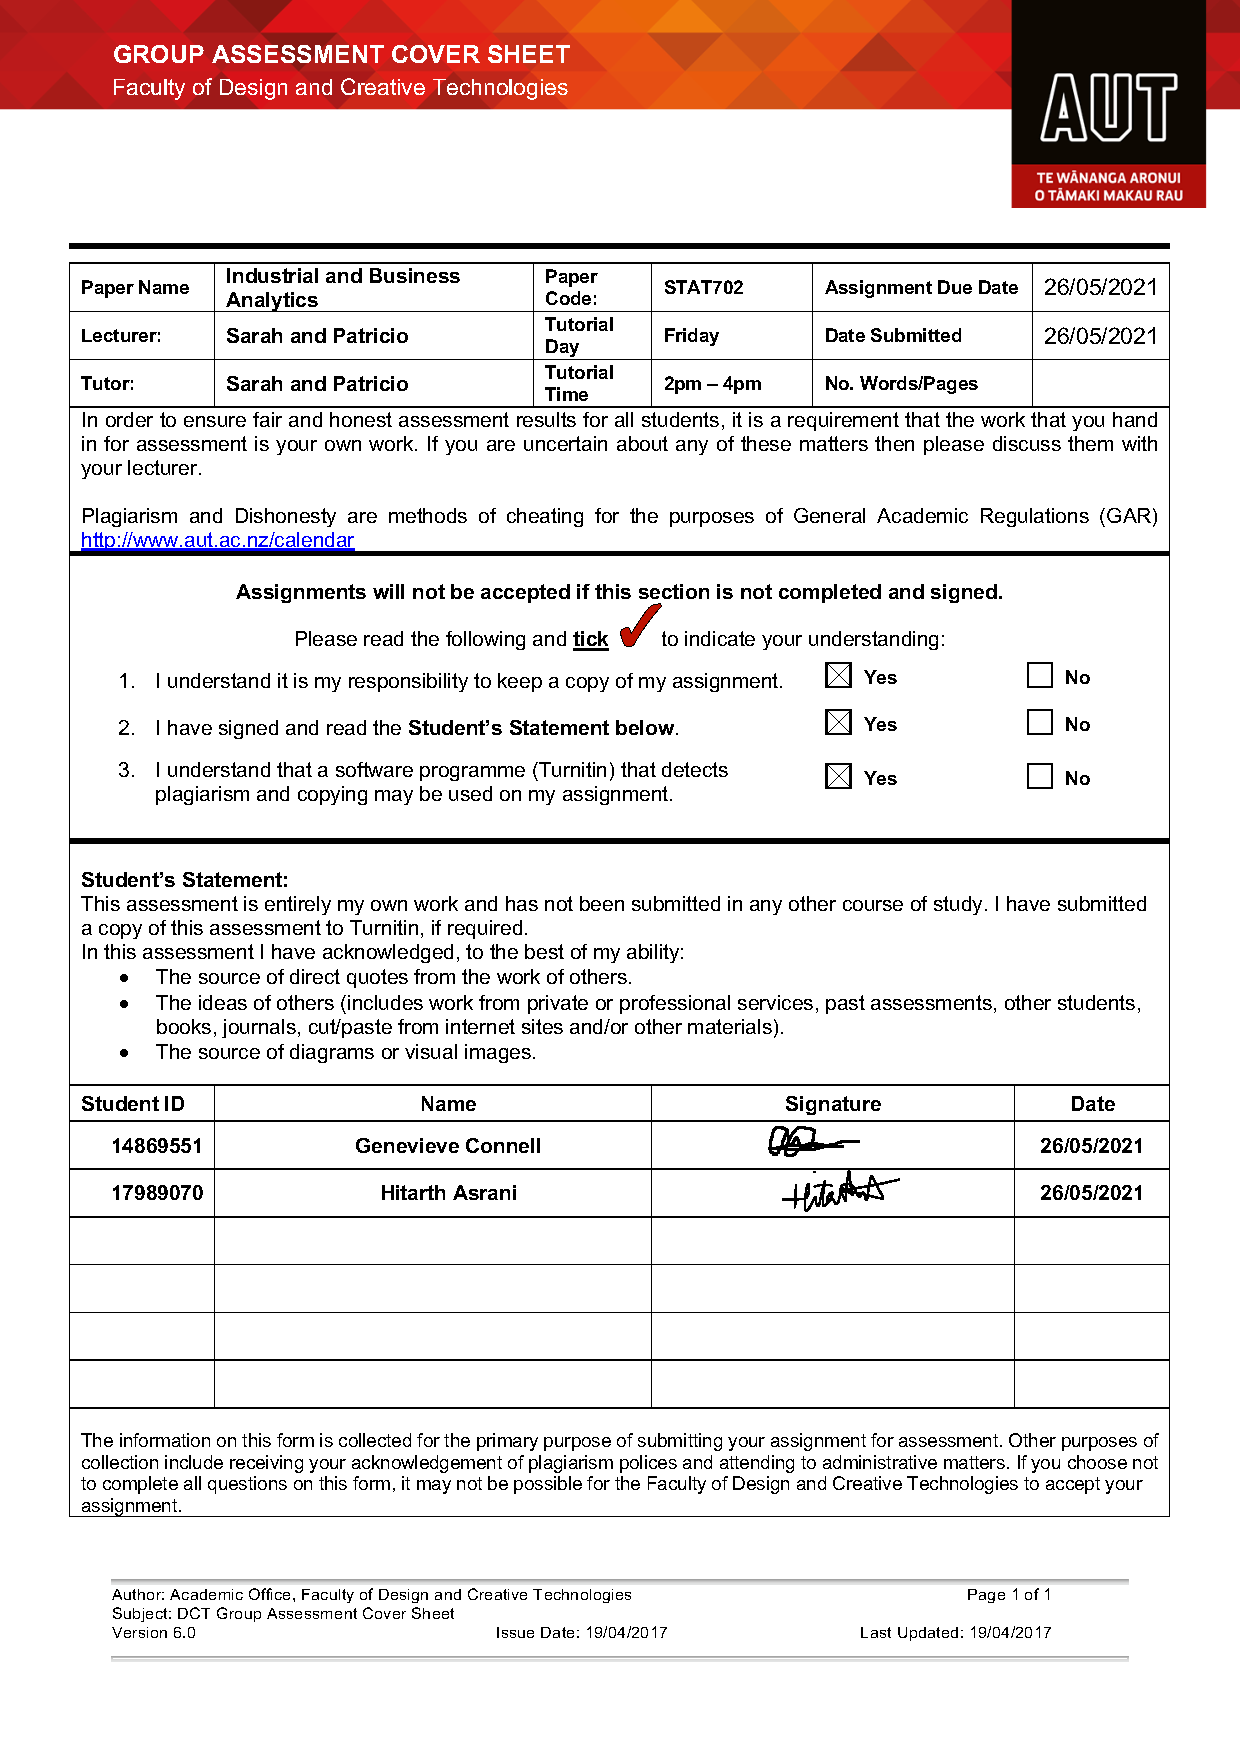
\includegraphics[width=15.5cm]{DCT-Group-Assessment-Cover-Sheet.pdf} \\[\bigskipamount] \newpage    \vspace*{3cm} \begin{center} \bf \LARGE} \posttitle{\end{center}  } \pagestyle{fancy} \fancyhf{} \renewcommand{\headrulewidth}{0pt} \fancyfoot[LE,RO]{\thepage}
\usepackage{float}
\ifluatex
  \usepackage{selnolig}  % disable illegal ligatures
\fi

\title{STAT702 Industrial and Business Analytics\\
Project}
\author{Genevieve Connell and Hitarth Asrani}
\date{25 May 2021}

\begin{document}
\maketitle

\newpage

\textbf{Group 5}: Hitarth Asrani and Genevieve Connell

\textbf{Product name}: BIC Round Stic Xtra Life Ballpoint Pen, Medium
Point (1.0mm), Red, 12-Count

\textbf{Sales sku\_id}: 219884

\textbf{Reviews asin}: B00006IE7J

\hypertarget{analysis-of-sales-data}{%
\section{1 Analysis of Sales Data}\label{analysis-of-sales-data}}

\hypertarget{a-for-the-product-sku_id-which-has-been-assigned-to-your-group-see-page-6-compute-the-total-monthly-sales-from-january-2011-july-2013.-present-your-results-in-an-appropriate-plot-and-write-2-3-sentences-describing-your-results.}{%
\subsection{1(a) For the product (sku\_id) which has been assigned to
your group (see page 6), compute the total monthly sales from January
2011 -- July 2013. Present your results in an appropriate plot and write
2 -- 3 sentences describing your
results.}\label{a-for-the-product-sku_id-which-has-been-assigned-to-your-group-see-page-6-compute-the-total-monthly-sales-from-january-2011-july-2013.-present-your-results-in-an-appropriate-plot-and-write-2-3-sentences-describing-your-results.}}

Hint: This will require some ``wrangling'' of the variable week. To do
this, format week as a date and then use the appropriate lubridate
function to extract the month.

Marking Criteria

\begin{itemize}
\item
  Total monthly sales have been correctly computed and are displayed in
  an appropriate plot.
\item
  Description of results/plot is correct and provides useful insights.
\item
  Plot is constructed using ggplot2 and has appropriate titles, labels,
  scales etc.**
\end{itemize}

\hypertarget{answer}{%
\subsection{Answer}\label{answer}}

From Jan 2011 - July 2013, 98434 units of sku 219844 were sold with a
mean monthly sale of 3175.3 and an interquartile range of 2621.5 -
3301.5.

Monthly sales are plotted below, no trend or seasonal pattern is evident
in this plot. There are three months with significantly high sales, May
2011, December 2011 and January 2012. The most significant outlier was
in January 2012 when 8871 units were sold. As shown in the plots below
these high monthly sales correspond with a high proportion of stores
featuring and/or displaying the product.

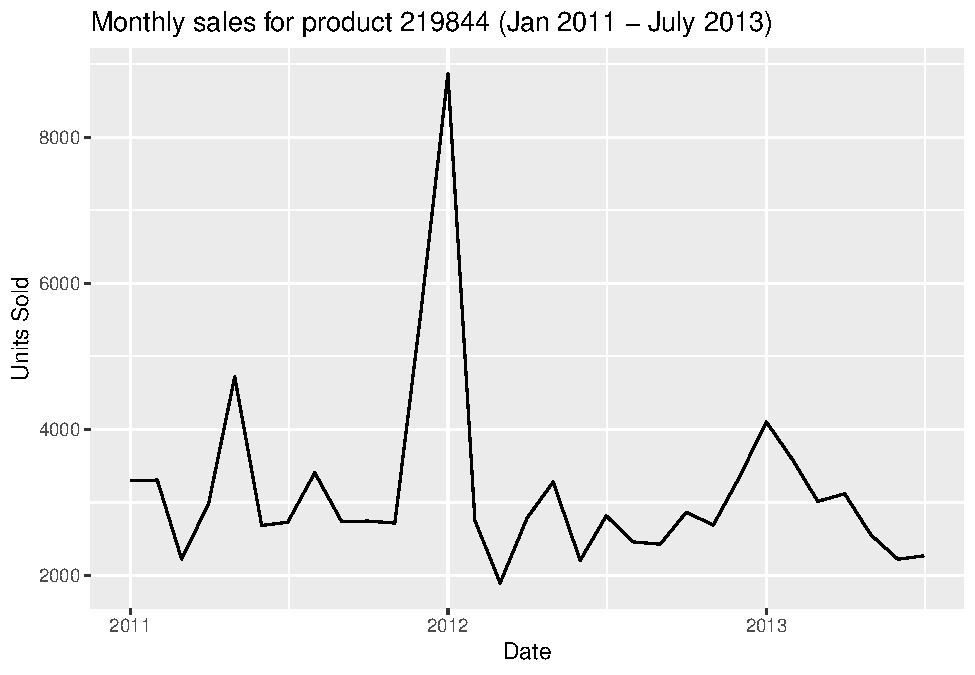
\includegraphics{Assignment-STAT702_files/figure-latex/1a plots-1.pdf}
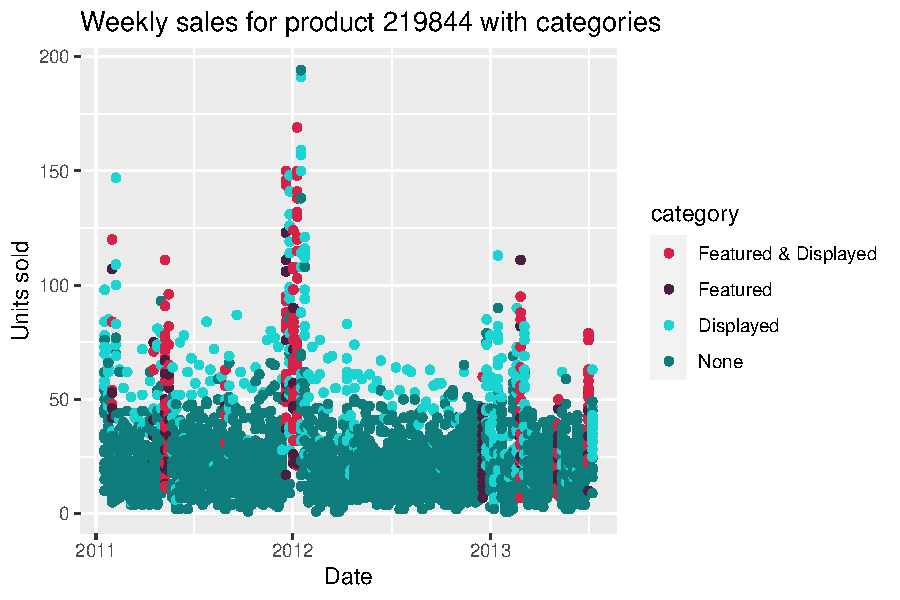
\includegraphics{Assignment-STAT702_files/figure-latex/1a plots-2.pdf}
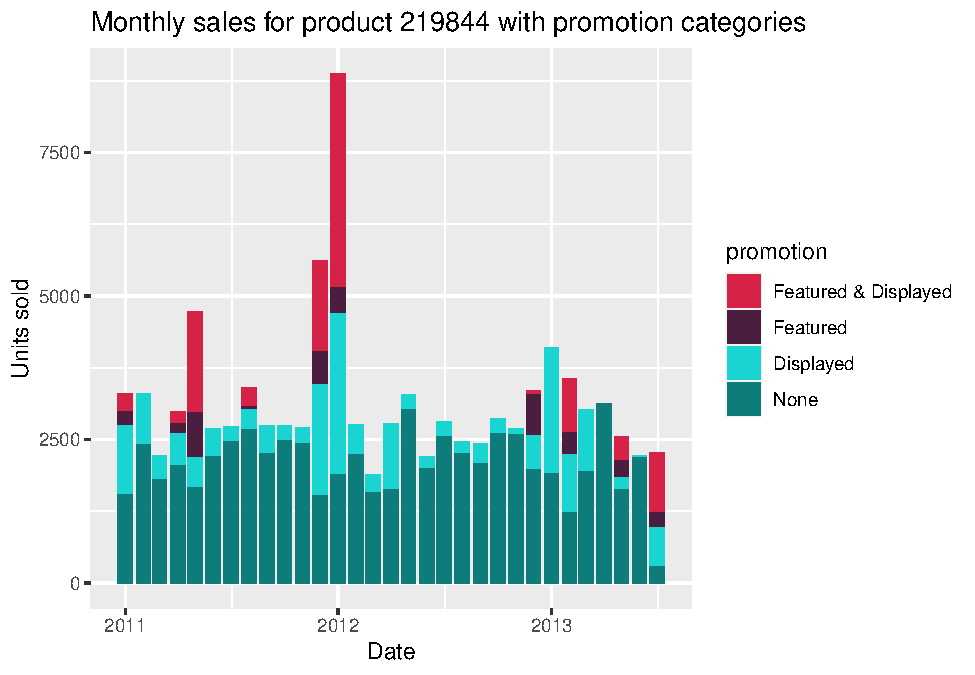
\includegraphics{Assignment-STAT702_files/figure-latex/1a plots-3.pdf}

\hypertarget{b-the-gm-sales-wants-to-know-which-stores-are-performing-well-and-which-are-not-in-terms-of-product-sales.-for-the-product-sku_id-which-has-been-assigned-to-your-group-use-appropriate-summary-statistics-and-plots-to-investigate-sales-performance-across-the-stores-and-write-2-3-paragraphs-summarising-your-findings.}{%
\subsection{1(b) The GM Sales wants to know which stores are performing
well and which are not, in terms of product sales. For the product
(sku\_id) which has been assigned to your group, use appropriate summary
statistics and plots to investigate sales performance across the stores
and write 2 -- 3 paragraphs summarising your
findings.}\label{b-the-gm-sales-wants-to-know-which-stores-are-performing-well-and-which-are-not-in-terms-of-product-sales.-for-the-product-sku_id-which-has-been-assigned-to-your-group-use-appropriate-summary-statistics-and-plots-to-investigate-sales-performance-across-the-stores-and-write-2-3-paragraphs-summarising-your-findings.}}

Hint: You will need to decide what it means for a store to be
``performing well'' and how you will evaluate this using the data.

Marking criteria

\begin{itemize}
\item
  Sales performance is clearly defined.
\item
  Written summary includes relevant and appropriate summary statistics
  and plots.
\item
  Plot/s are constructed using ggplot2 and have appropriate titles,
  labels, scales etc.
\item
  Descriptions of results and plots are correct and provides useful
  insights.
\end{itemize}

\hypertarget{answer-1}{%
\subsection{Answer}\label{answer-1}}

All stores have been ranked based on their total sales from Jan 2011 to
July 2013. The store with the highest total units sold is ranked `1',
this is store 9279 with 6698 units.

Below is a bar chart showing the total units sold with stores ordered by
rank. Sales for 2013 are much lower than 2011 and 2012 as only half the
years data is included.

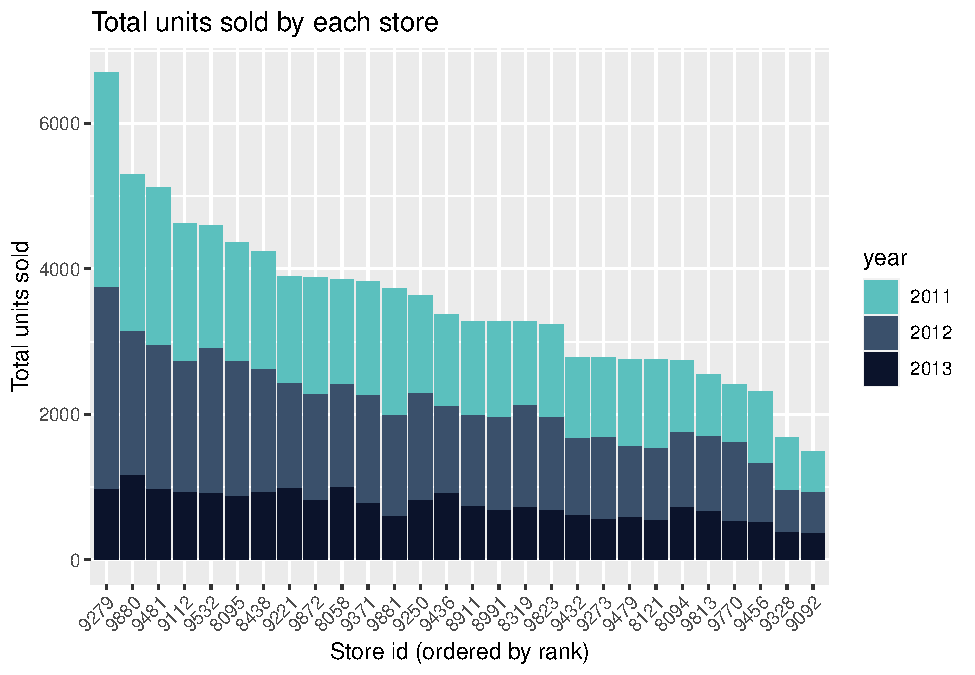
\includegraphics{Assignment-STAT702_files/figure-latex/1b store totals-1.pdf}

For a more detailed look at store performance monthly sales have been
plotted for each store and categorised as `High', `Average' or `Low'
performing. These categories are based on the interquartile range for
monthly sales. This range is 71 - 138 and captures 50\% of all monthly
sales. Monthly sales within the range are classified as `Average', sales
greater than 138 are classified as `High' performing and those below 71
are classified as `Low' performing.

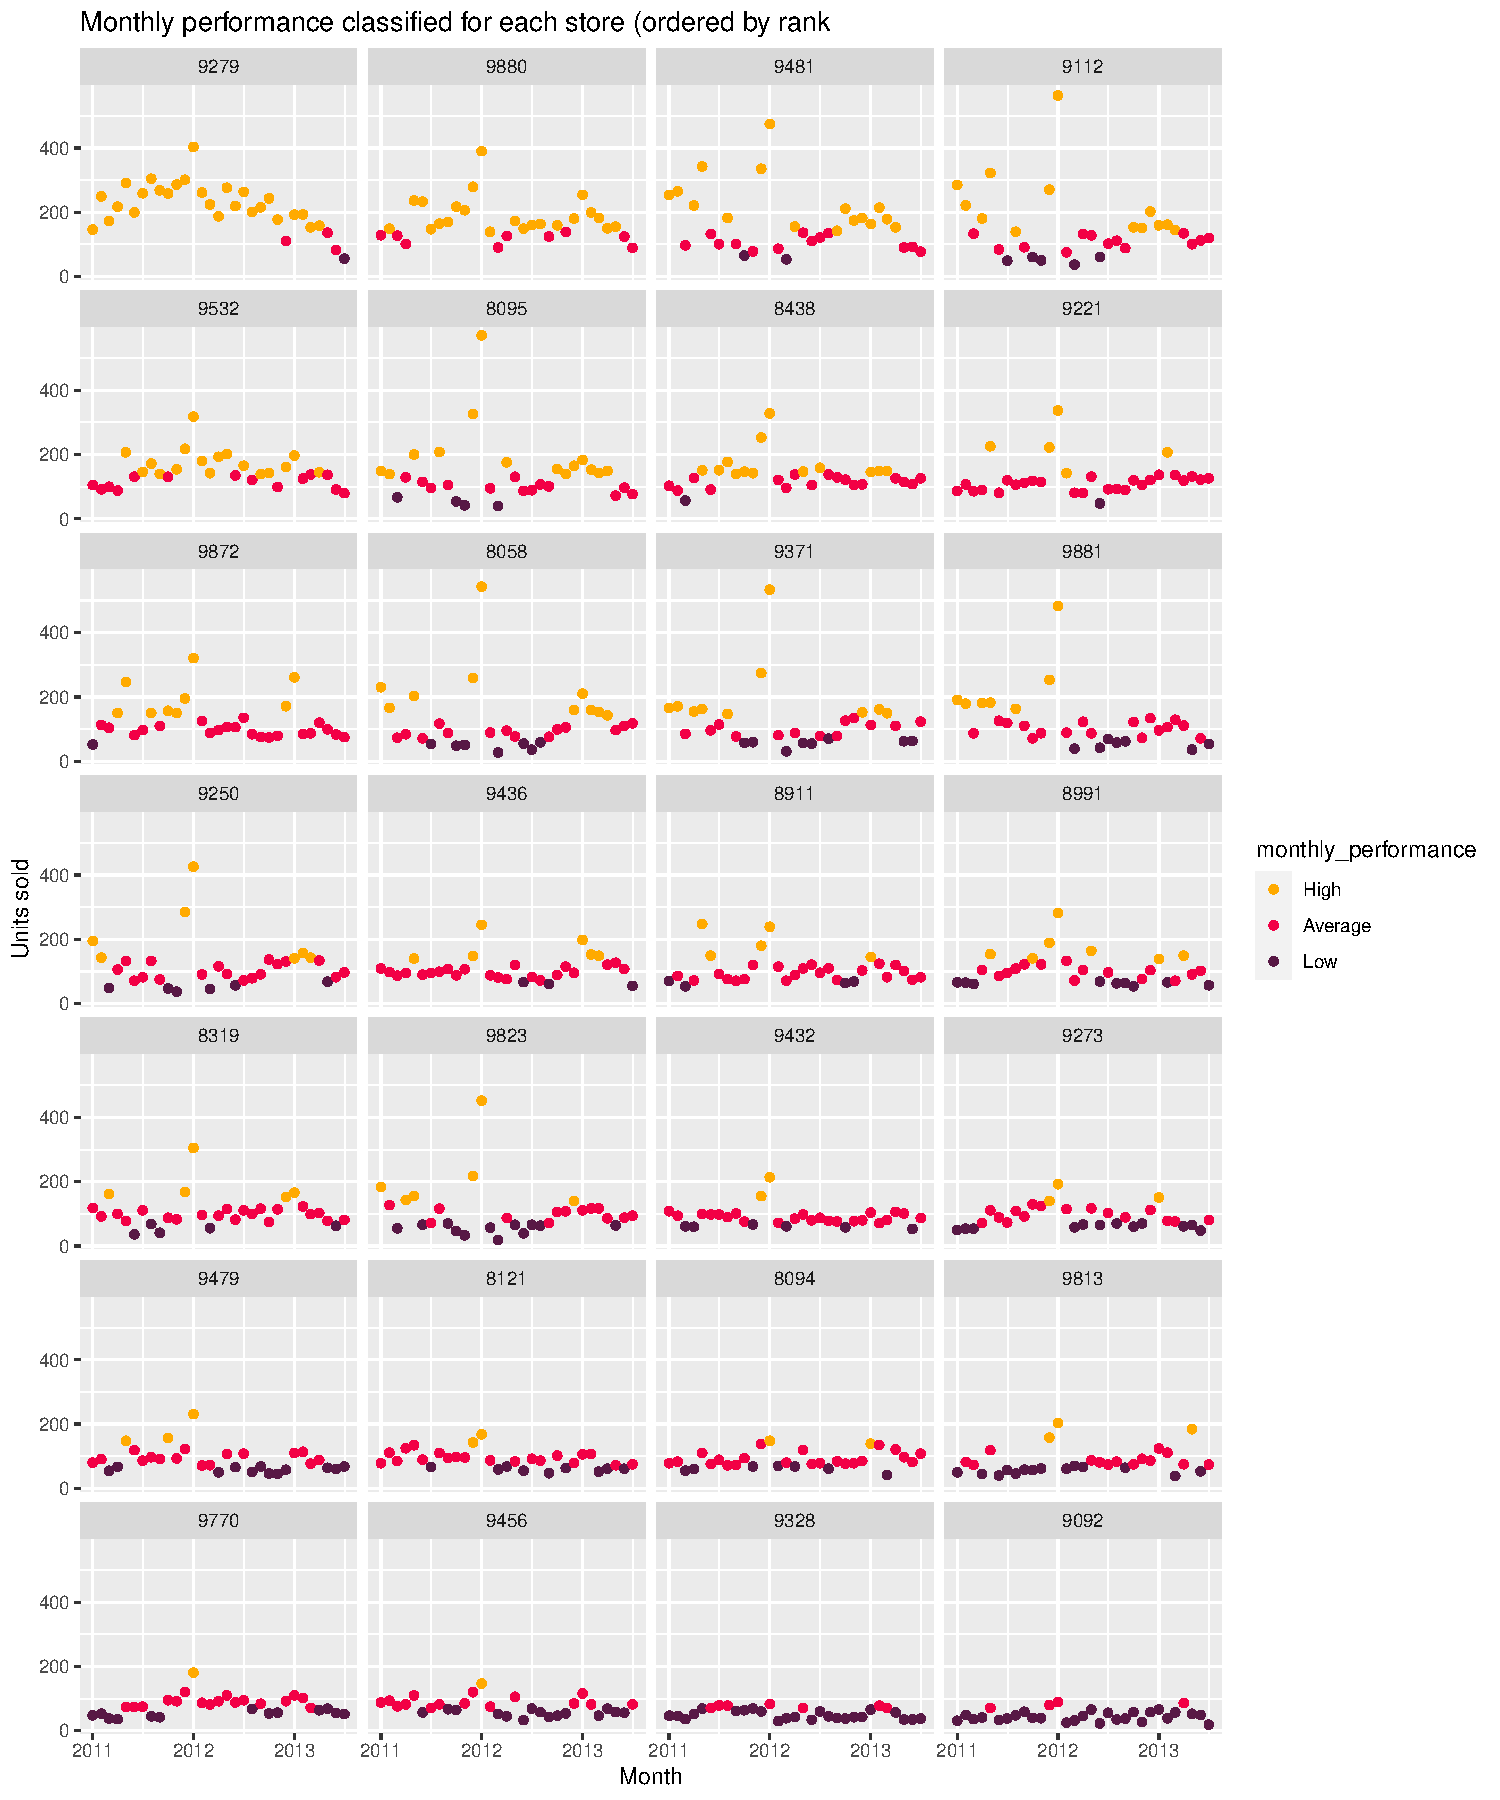
\includegraphics{Assignment-STAT702_files/figure-latex/store plots-1.pdf}

An interesting feature of these plots is that some stores have more
consistent performance than others. For example store 9112 had 5 low
performing months but was ranked at 4, much higher than store 9872 which
had only 1 low performing month but was ranked 9. Despite having higher
overall sales store 9112 was less reliably successful than store 9872.

Stores with high occurrences of low sales are not reliable and are a
source of risk. As an alternative to ranking stores based on their
overall sales, stores have been given a ranking based on their
consistency. For every high performing month stores are given a score of
3, for every average month a score of 2 and for every low performing
month a score of 1.

Below is a plot showing stores ordered according to the new consistency
rank along with the number of High, Average and Low performing months
they achieved. Another plot is included for comparison where stores are
ranked according to overall sales. Under the new consistency ranking
scheme stores with unreliable performance such as 9112 drop in rank
whilst stores with reliable performance such as 9532 are ranked more
highly.

Overall consistency ranking seems most appropriate for sales performance
as it rewards stores with reliable monthly sales. Consistency ranking
has been used to split stores into three groups of overall performance.
The top third of stores (consistency rank 1-9) are evaluated as `High'
performing. The middle third of stores (rank 10-18) are evaluated as
having `Average' performance and stores in the bottom third (rank 19-28)
are evaluated as `Low' performing.

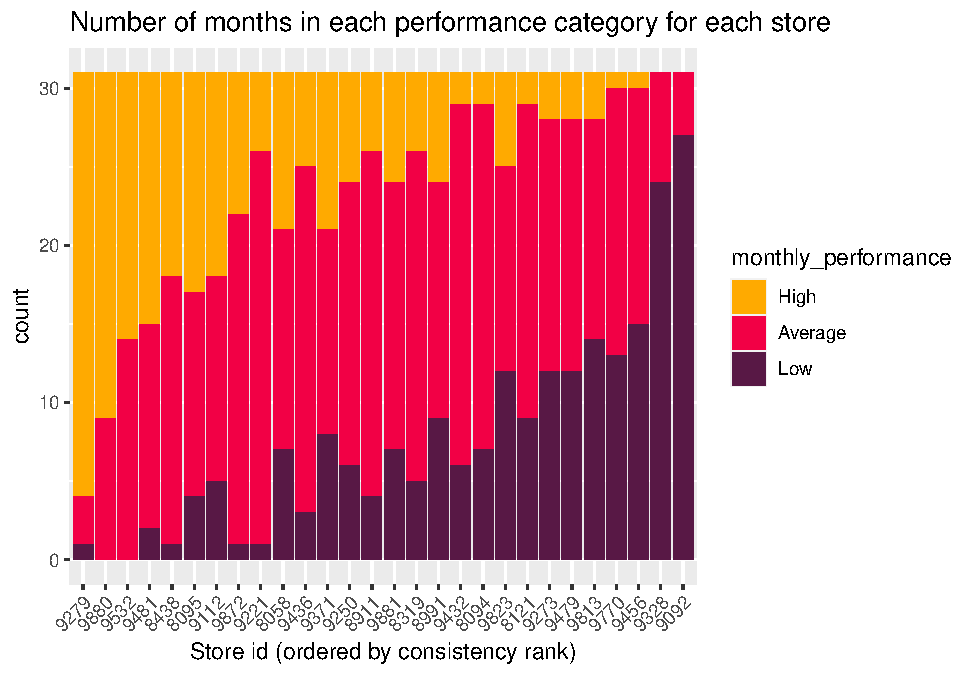
\includegraphics{Assignment-STAT702_files/figure-latex/promotion_plots-1.pdf}
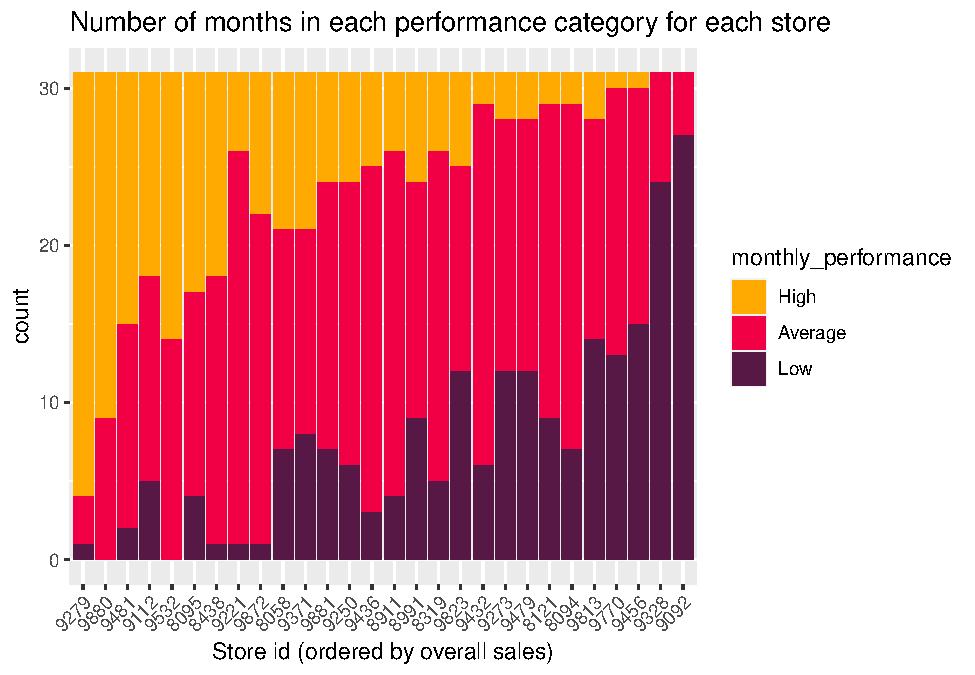
\includegraphics{Assignment-STAT702_files/figure-latex/promotion_plots-2.pdf}

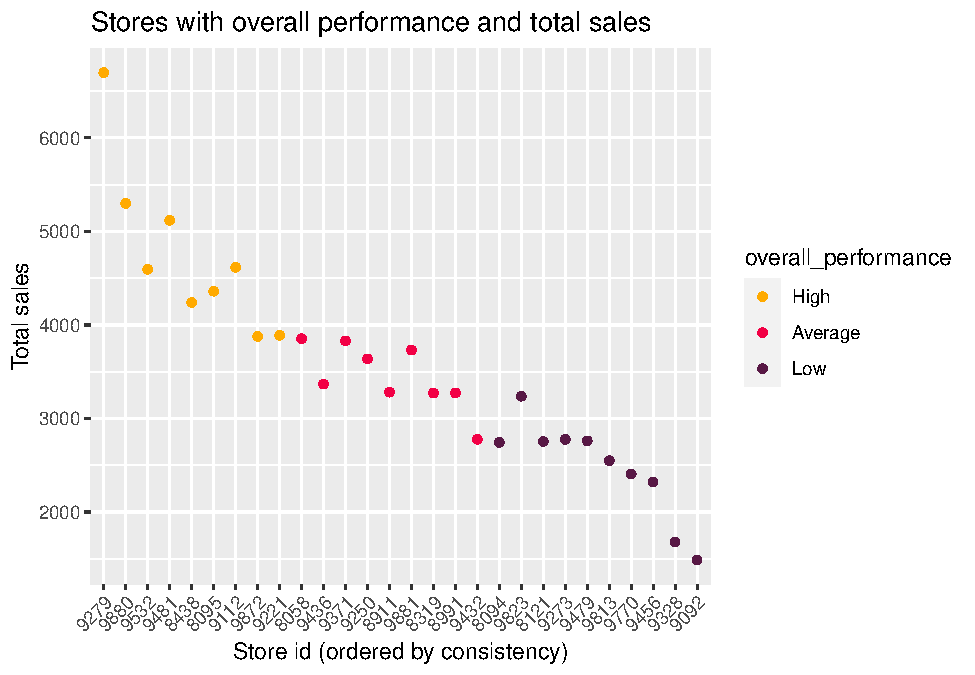
\includegraphics{Assignment-STAT702_files/figure-latex/unnamed-chunk-1-1.pdf}

Below is a plot showing that when a product is featured and/or displayed
weekly sales are more likely to be high. Weekly performance has been
categorised into `High', `Average' and `Low' based on the interquartile
range of weekly sales. When the product is featured and/or displayed a
higher proportion of weekly sales have been `High' or `Average' compared
to no promotion.

Low performing stores could boost their sales by increasing the number
of weeks they promote the product and unreliable stores could ensure
high sales by holding regular promotions.

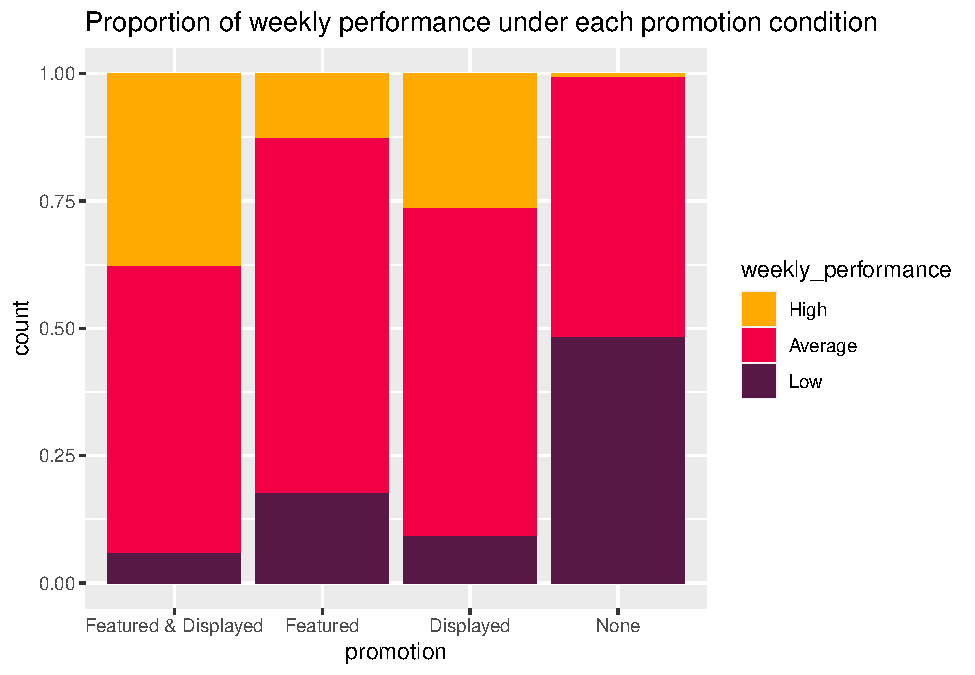
\includegraphics{Assignment-STAT702_files/figure-latex/1b-1.pdf}

\hypertarget{question-2}{%
\section{Question 2}\label{question-2}}

\hypertarget{a-the-operations-manager-is-interested-in-studying-an-eoq-model-for}{%
\subsection{(a) The Operations Manager is interested in studying an EOQ
model
for}\label{a-the-operations-manager-is-interested-in-studying-an-eoq-model-for}}

\begin{verbatim}
product 216233, based on sales in 2012. The setup and holding costs
are known to be 130 per order and 1.50 per unit per year,
respectively.
\end{verbatim}

\hypertarget{i-determine-the-best-order-quantity-in-such-a-way-that-the-costs-are-minimised.-write-1-2-paragraphs-summarising-your-findings.}{%
\subsection{i) Determine the best order quantity in such a way that the
costs are minimised. Write 1 -- 2 paragraphs summarising your
findings.}\label{i-determine-the-best-order-quantity-in-such-a-way-that-the-costs-are-minimised.-write-1-2-paragraphs-summarising-your-findings.}}

Marking criteria

• Number of orders during a year, number of days between orders, and the
total annual inventory cost are correctly computed and included in the
findings.

• The paragraphs clearly explain your findings.

• Assumptions of the EOQ model are clearly stated

The Economic Order Quantity (EOQ) model is used to find the best order
quantity so that total costs are minimised. Key assumptions to this
model are that demand is constant and known, there is no lead time,
orders arrive instantaneously and back orders are not allowed. Another
assumption is that stock levels are under continuous review.

Demand for product 216233 has been estimated based on the annual demand
from 2012, this is 169591. The optimum order quantity is calculated
based on this demand and the annual order and holding costs. The
following EOQ formula is used to determine optimal order quantity where
k is order cost and h is holding cost.

\[Q^* =  \sqrt{\frac{2kA}{h}}\] The optimal order quantity is calculated
to be 5422 with an inventory cycle of 12 days. This means that every 12
days 5422 units are ordered, resulting in 31 annual orders. This model
results in the smallest possible annual inventory cost of 8132.6803762
with an annual order cost of 4066.1803762 and an annual holding cost of
4066.5. This EOQ model is plotted for two cycles below.

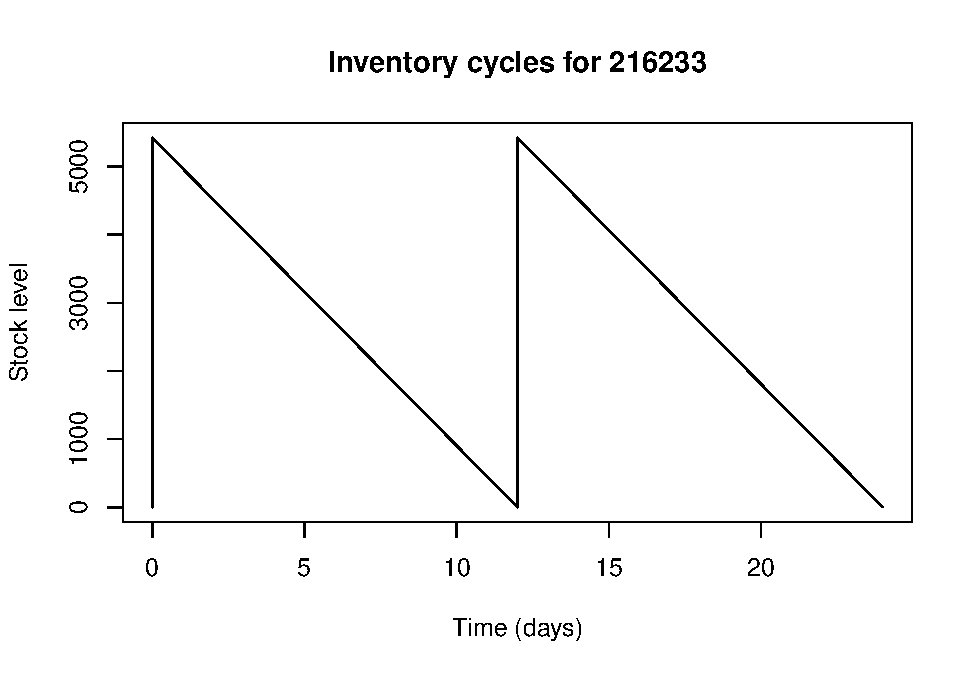
\includegraphics{Assignment-STAT702_files/figure-latex/2ai plot-1.pdf}

\hypertarget{ii-the-operations-manager-is-also-interested-in-studying-a-model-in-which-backorders-are-permitted.-according-to-its-estimates-the-cost-of-backorders-is-approximately-5-of-the-total-price-price-per-unit.-determine-the-best-order-quantity-in-the-sense-that-inventory-costs-are-minimised.-write-1-2-paragraphs-summarising-your-findings-and-plot-the-first-two-inventory-cycles.}{%
\subsection{ii) The Operations Manager is also interested in studying a
model in which backorders are permitted. According to its estimates, the
cost of backorders is approximately 5\% of the total price (price per
unit). Determine the best order quantity in the sense that inventory
costs are minimised. Write 1 -- 2 paragraphs summarising your findings
and plot the first two inventory
cycles.}\label{ii-the-operations-manager-is-also-interested-in-studying-a-model-in-which-backorders-are-permitted.-according-to-its-estimates-the-cost-of-backorders-is-approximately-5-of-the-total-price-price-per-unit.-determine-the-best-order-quantity-in-the-sense-that-inventory-costs-are-minimised.-write-1-2-paragraphs-summarising-your-findings-and-plot-the-first-two-inventory-cycles.}}

• The optimum order quantity, maximum level of stock, optimum time
between orders, proportion of time the company have to take backorders,
and total annual inventory cost are correctly computed and included in
your answer.

• The paragraphs clearly explain your findings.

• Assumptions of the model are clearly stated.

• The first two inventory cycles are correctly plotted

The Optimum Backorder Model is used to find the best order quantity so
that total costs are minimised when backorders are allowed. Similar to
the EOQ model assumptions are made that demand is constant and known,
there is no lead time, orders arrive instantaneously and stock levels
are under continuous review.

Annual demand is estimated as 169591 using 2012 data. Backorders cost is
approximately 5\% of the total price per unit. In the 2012 sales data
total price for product 216233 varies from 78.4 to 134.7. For evaluating
the backorder cost the mean total price 78.4 has been used, resulting in
a backorder cost (p) of 6.22 per unit. The optimum quantity \((Q^*)\)
and optimum maximum inventory level \((S^*)\) are calculated using the
following forumlas.

\[Q^* = \sqrt{\frac{2kA}{h}} \sqrt{\frac{p+h}{p}} \]
\[S^* = \sqrt{\frac{2kA}{h}} \sqrt{\frac{p}{p+h}} \] Optimal order
quantity is calculated to be 6040 with an inventory cycle of 13 days.
This means that every 13 days 6040 units are ordered, resulting in 28
annual orders. The optimum inventory level is 4867 and the proportion of
time taking back orders is 23\%. This model results in the smallest
possible annual inventory cost of 7300.44 with an annual order cost of
3650.14 and an annual holding cost of 2941.35 and annual backorder cost
of 709. This EOQ model is plotted for two cycles below.

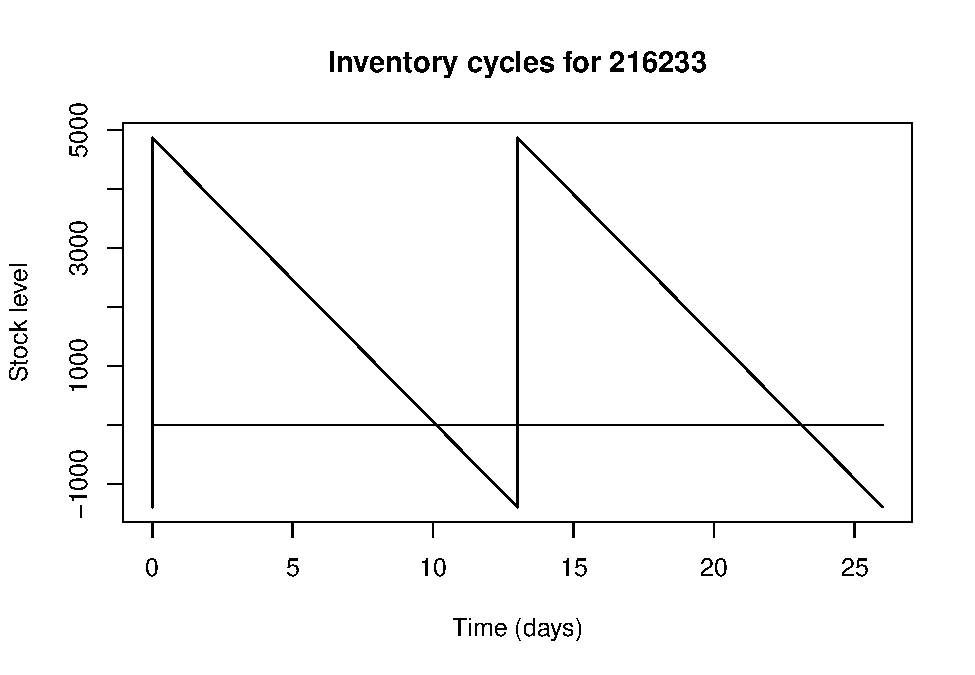
\includegraphics{Assignment-STAT702_files/figure-latex/2aii plot-1.pdf}

\hypertarget{iii-plot-the-inventory-cycles-associated-with-the-model-in-part-ii-and-compare-with-the-observed-inventory-levels-in-2012-assuming-actual-demand-during-2012-and-the-order-frequency-and-order-quantity-from-the-model.-write-2-3-sentences-describing-your-plot.}{%
\subsection{iii) Plot the inventory cycles associated with the model in
part ii and compare with the observed inventory levels in 2012, assuming
actual demand during 2012, and the order frequency and order quantity
from the model. Write 2 -- 3 sentences describing your
plot.}\label{iii-plot-the-inventory-cycles-associated-with-the-model-in-part-ii-and-compare-with-the-observed-inventory-levels-in-2012-assuming-actual-demand-during-2012-and-the-order-frequency-and-order-quantity-from-the-model.-write-2-3-sentences-describing-your-plot.}}

• The inventory levels from the model and data are correctly plotted.

• Accurate and insightful comments are made about the plot.

• Note: This is a bonus question. The maximum mark that could be awarded
for this project is 100

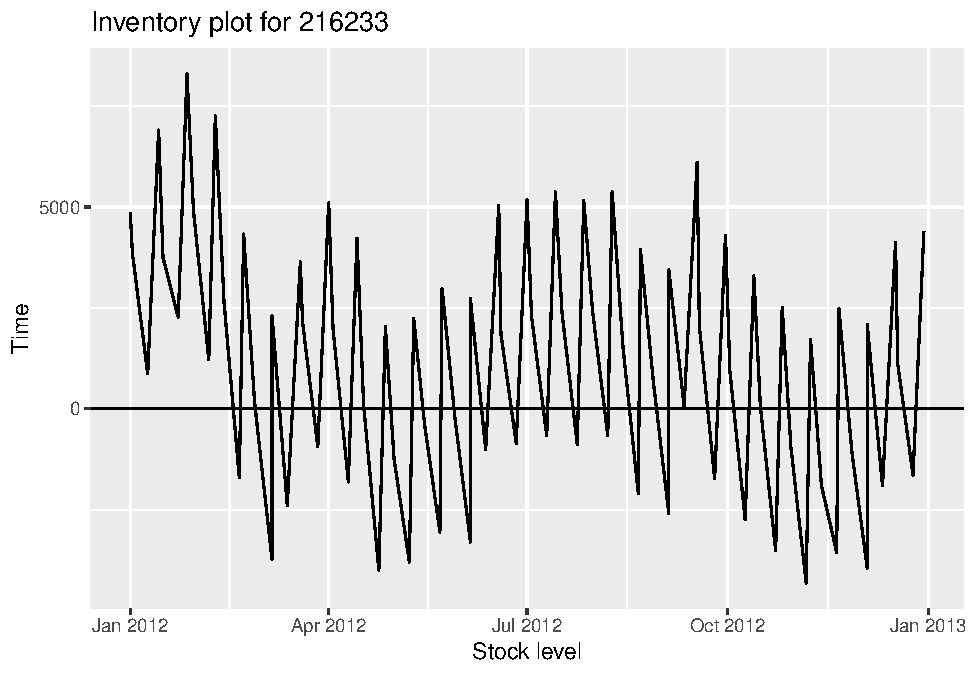
\includegraphics{Assignment-STAT702_files/figure-latex/2aiii-1.pdf}

The plot above shows the weekly demand from the 2012 sales data plotted
with the optimum order frequency, 13 days and optimum order quantity
6040 from the Optimum Backorder Model. Stock starts at the optimum
inventory level 4867, decreases with every weekly sale quantity from
2012 data and increases with inventory added at the optimum frequency
and quantity.

Actual demand is not constant and as a result the quantity and frequency
found with the back order model is not always appropriate. The model
performs best when demand is constant, for example in July.

\hypertarget{b}{%
\section{2b}\label{b}}

The Operations Manager is considering the option of a multi-period
inventory model. The company, as a policy, is not willing to tolerate
more than 5\% chance of a stock-out. The Operations Manager has
estimated that the annual holding cost is 6.50 per unit and the ordering
cost is 20.50 per order.

\hypertarget{i.-calculate-a-multi-period-inventory-model-for-product-216425-based-on-the-2012-sales-data.-create-plots-of-the-weekly-average-demand-of-this-product.-use-the-costs-stated-in-part-babove.-write-a-paragraph-explaining-the-results-of-your-model-and-the-plots.}{%
\subsection{i. Calculate a multi-period inventory model for product
216425, based on the 2012 sales data. Create plot/s of the weekly
average demand of this product. Use the costs stated in part (b)above.
Write a paragraph explaining the results of your model and the
plot/s.}\label{i.-calculate-a-multi-period-inventory-model-for-product-216425-based-on-the-2012-sales-data.-create-plots-of-the-weekly-average-demand-of-this-product.-use-the-costs-stated-in-part-babove.-write-a-paragraph-explaining-the-results-of-your-model-and-the-plots.}}

Hint: Use the weekly demand to estimate the demand during a one-week
lead time.

• The optimal order quantity, safety stock, expected annual cost, orders
per years are correctly computed and included in your answer.

• The paragraph clearly explains your findings.

• The assumption of normality for the demand during a one-week lead time
is discussed.

• The weekly average demand of this product is correctly plotted and
discussed

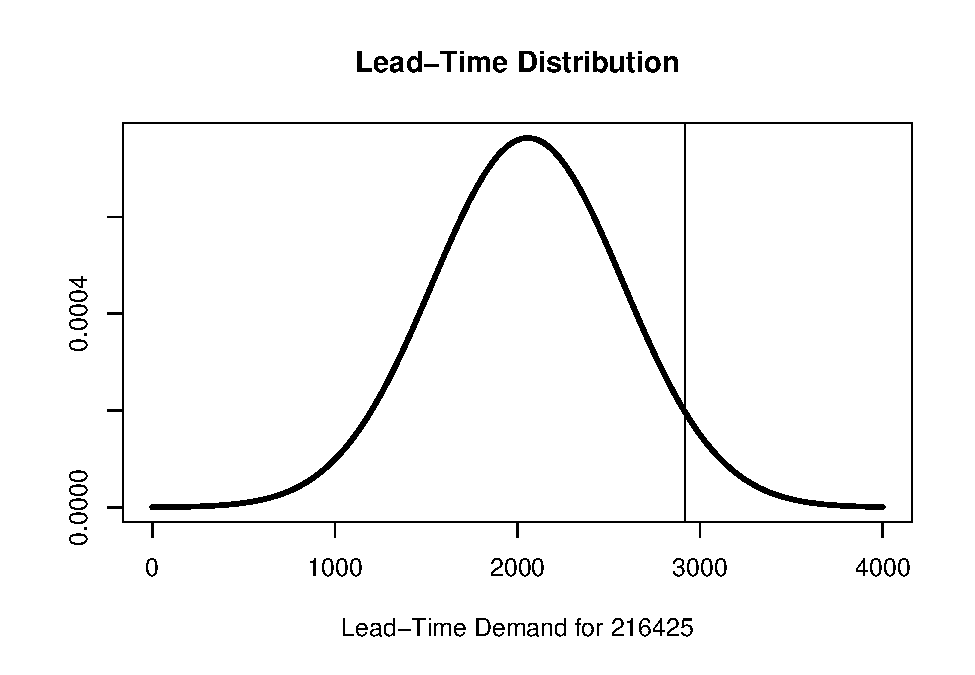
\includegraphics{Assignment-STAT702_files/figure-latex/2bi-1.pdf}

\begin{verbatim}
## integer(0)
\end{verbatim}

For this multi-inventory model demand during a one week lead time has
been estimated using the mean and standard deviation of observed data in
2012. Demand has been estimated as a normal distribution with a mean of
2057 and standard deviation of 523. As the plot below shows, whilst the
actual demand for 2012 does not perfectly follow this distribution it is
a adequate approximation.

The expected annual demand is estimated to be 106939. Given this annual
demand and the costs of holding and reordering stock, the recommended
multi-inventory model is to order 821 units whenever the order quantity
reaches the reorder point of 2916 units. Approximately 130 orders will
be placed per year and safety stock is 821. This approach ensures
roughly 95\% of the time stock will be sufficient for weekly demand. The
expected annual costs are 10926.7492 per year. If demand was certain the
annual costs would only be 5338.4686358 so the additional cost of
holding safety stock is 5588.2805642.

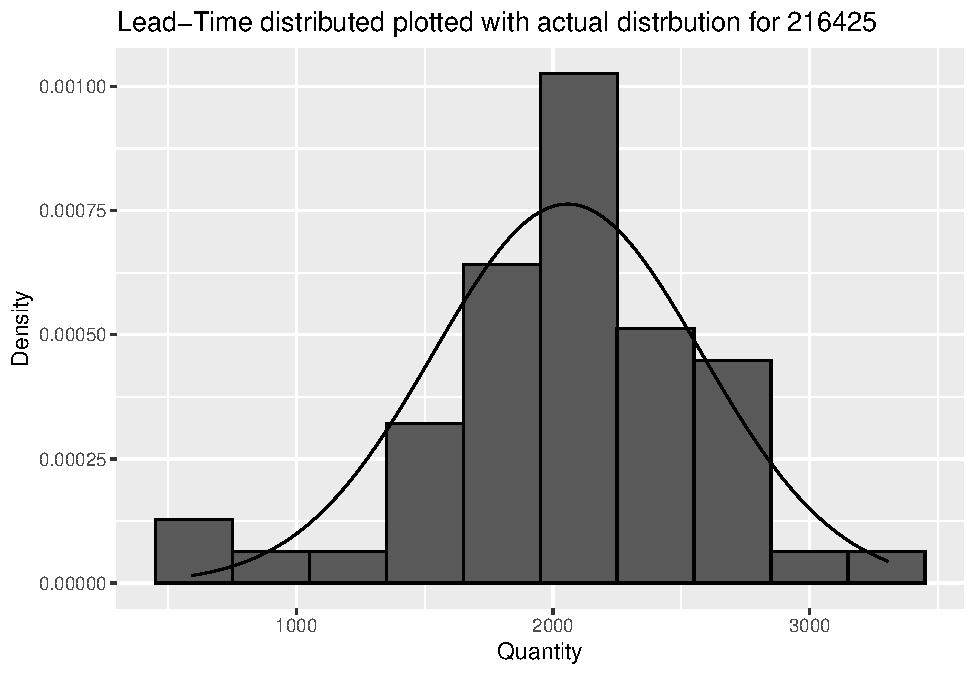
\includegraphics{Assignment-STAT702_files/figure-latex/2bi plot-1.pdf}

\hypertarget{b.ii.-investigate-the-use-of-a-multi-period-inventory-model-for-the-product-which-has-been-assigned-to-your-group-based-on-the-2012-sales-data.-create-plots-of-the-weekly-average-demand-of-this-product.-use-the-costs-stated-in-part-b-above.}{%
\subsection{2.b.ii. Investigate the use of a multi-period inventory
model for the product which has been assigned to your group, based on
the 2012 sales data. Create plot/s of the weekly average demand of this
product. Use the costs stated in part (b)
above.}\label{b.ii.-investigate-the-use-of-a-multi-period-inventory-model-for-the-product-which-has-been-assigned-to-your-group-based-on-the-2012-sales-data.-create-plots-of-the-weekly-average-demand-of-this-product.-use-the-costs-stated-in-part-b-above.}}

\hypertarget{discuss-the-assumptions-of-the-model-and-suggest-a-solution-in-case-of-finding-any-problems.-write-a-paragraph-explaining-the-results-of-your-findings-and-the-plot.}{%
\subsection{Discuss the assumptions of the model and suggest a solution,
in case of finding any problems. Write a paragraph explaining the
results of your findings and the
plot.}\label{discuss-the-assumptions-of-the-model-and-suggest-a-solution-in-case-of-finding-any-problems.-write-a-paragraph-explaining-the-results-of-your-findings-and-the-plot.}}

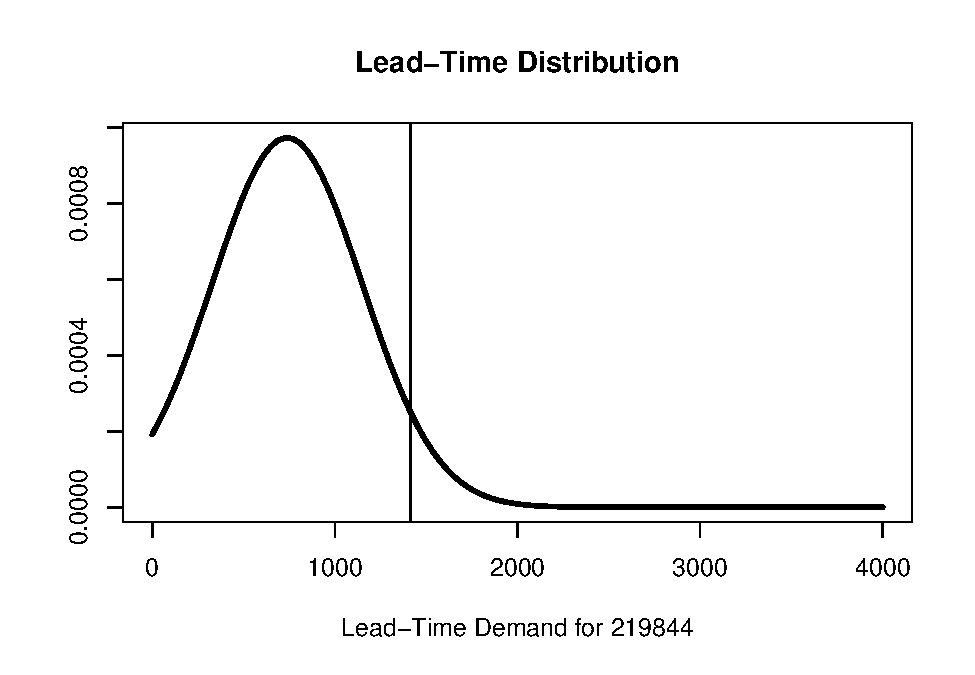
\includegraphics{Assignment-STAT702_files/figure-latex/2bii-1.pdf}

\begin{verbatim}
## integer(0)
\end{verbatim}

For this multi-inventory model demand during a one week lead time has
been estimated using the mean and standard deviation of observed data in
2012. Demand has been estimated as a normal distribution with a mean of
739 and standard deviation of 410. As the plot below shows this
distribution is a very poor fit for the observed data. It is recommended
that a more accurate distribution is used for estimating the Lead-Time
distribution and reorder point. It is likely that the reorder point
calculated with this normal distribution is unnecessarily high.

The expected annual demand is estimated to be 38410. Given this annual
demand and the costs of holding and reordering stock, the recommended
multi-inventory model is to order 492 units whenever the order quantity
reaches the reorder point of 1413 units. Approximately 78 orders will be
placed per year and safety stock is 492. This approach ensures roughly
95\% of the time stock will be sufficient for weekly demand. The
expected annual costs are 7582.3685882 per year. If demand was certain
the annual costs would only be 3199.4166667 so the additional cost of
holding safety stock is 4382.9519216.

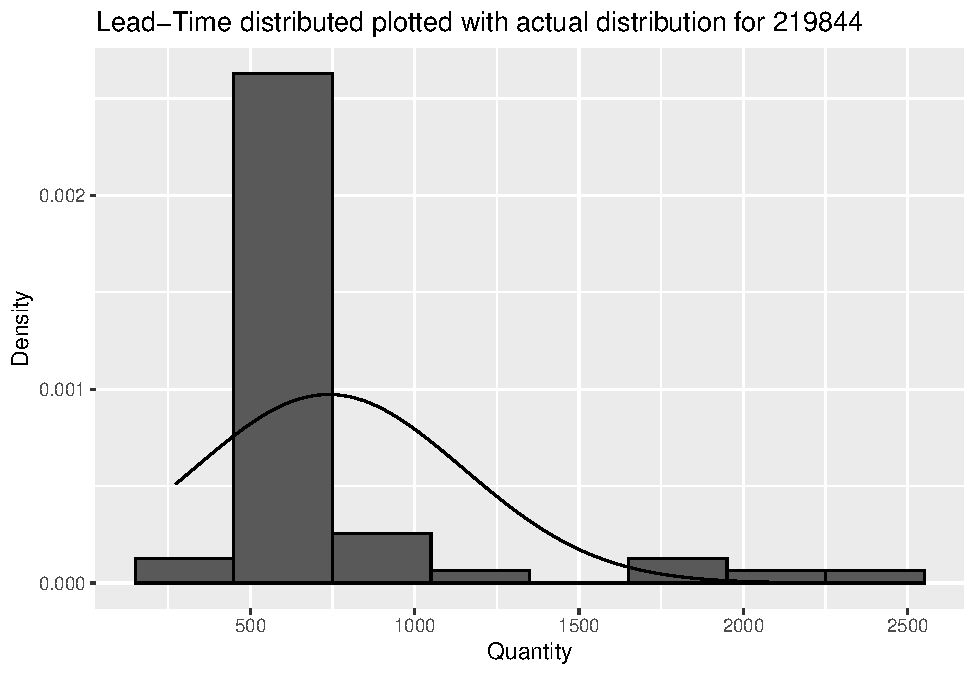
\includegraphics{Assignment-STAT702_files/figure-latex/2bii plot-1.pdf}

\hypertarget{question-3}{%
\section{Question 3}\label{question-3}}

\hypertarget{a-for-the-product-asin-that-has-been-assigned-to-your-group-use-summary-statistics-and-plots-to-analyse-the-overall-review-rating-overall.-write-a-paragraph-describing-your-findings-to-the-general-manager---sales.}{%
\subsection{a) For the product (asin) that has been assigned to your
group, use summary statistics and plots to analyse the overall review
rating (overall). Write a paragraph describing your findings to the
General Manager -
sales.}\label{a-for-the-product-asin-that-has-been-assigned-to-your-group-use-summary-statistics-and-plots-to-analyse-the-overall-review-rating-overall.-write-a-paragraph-describing-your-findings-to-the-general-manager---sales.}}

Marking Criteria • Summary statistics for the overall review rating have
been correctly computed and are displayed in appropriate plot/s.

• Descriptions of results and plots are correct and provide useful
insights.

• Plot/s are constructed using ggplot2 and have appropriate
titles,labels,scalesetc.

\hypertarget{answer-2}{%
\subsection{Answer}\label{answer-2}}

Reviews were rated from 1-5. The mean rating for product B00006IE7J is
4.7. Most reviews were rated highly with 79 given 5 and 13.4 given 4
stars.

\begin{longtable}[]{@{}llllll@{}}
\toprule
Min & 1st Qu. & Median & Mean & 3rd Qu. & Max \\
\midrule
\endhead
1 & 5 & 5 & 4.7 & 5 & 5 \\
\bottomrule
\end{longtable}

Some reviews were verified and others were not. The proportion of
ratings given by these different groups are compared below. The
unverified group gave a higher proportion of ratings 2-4 than the
verified group.

Review ratings have been plotted below against time. Most reviews were
given between 2014 and 2018. Rating does not appear to be strongly
correlated with time.

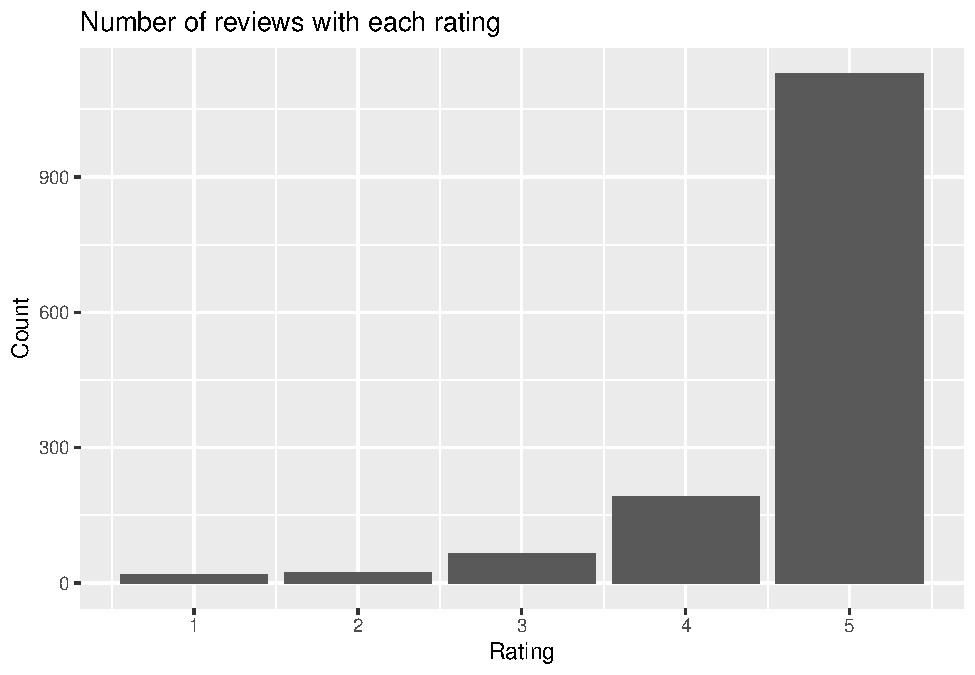
\includegraphics{Assignment-STAT702_files/figure-latex/3a plots-1.pdf}
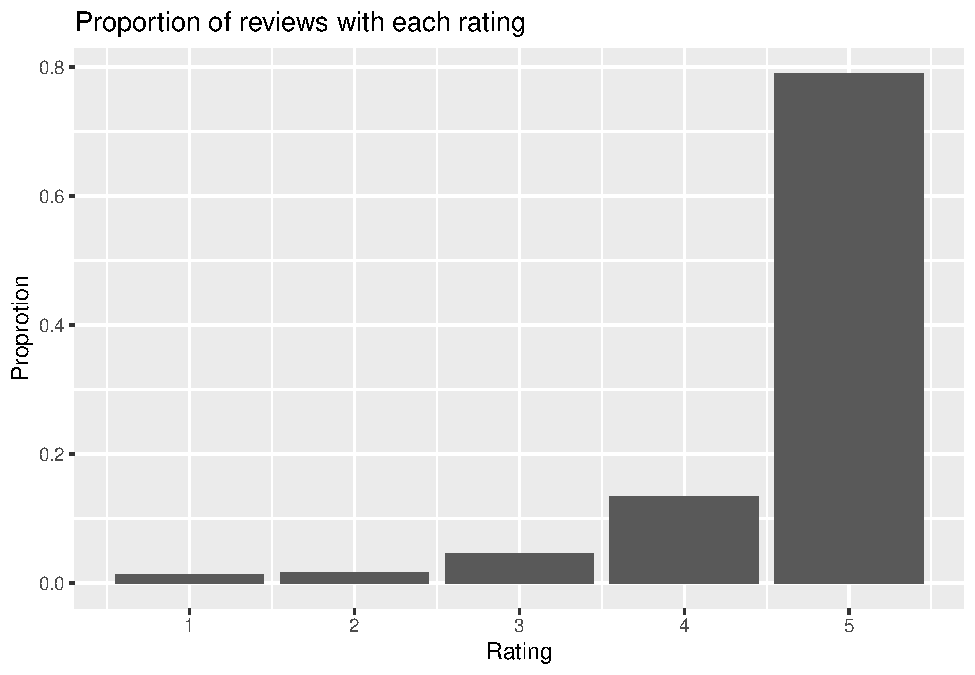
\includegraphics{Assignment-STAT702_files/figure-latex/3a plots-2.pdf}
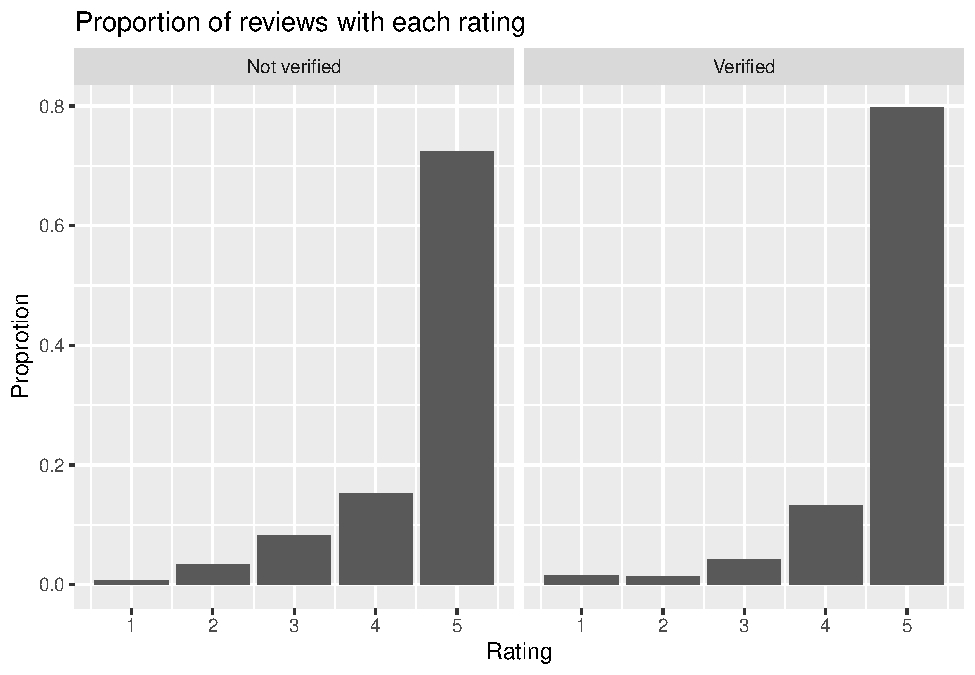
\includegraphics{Assignment-STAT702_files/figure-latex/3a plots-3.pdf}
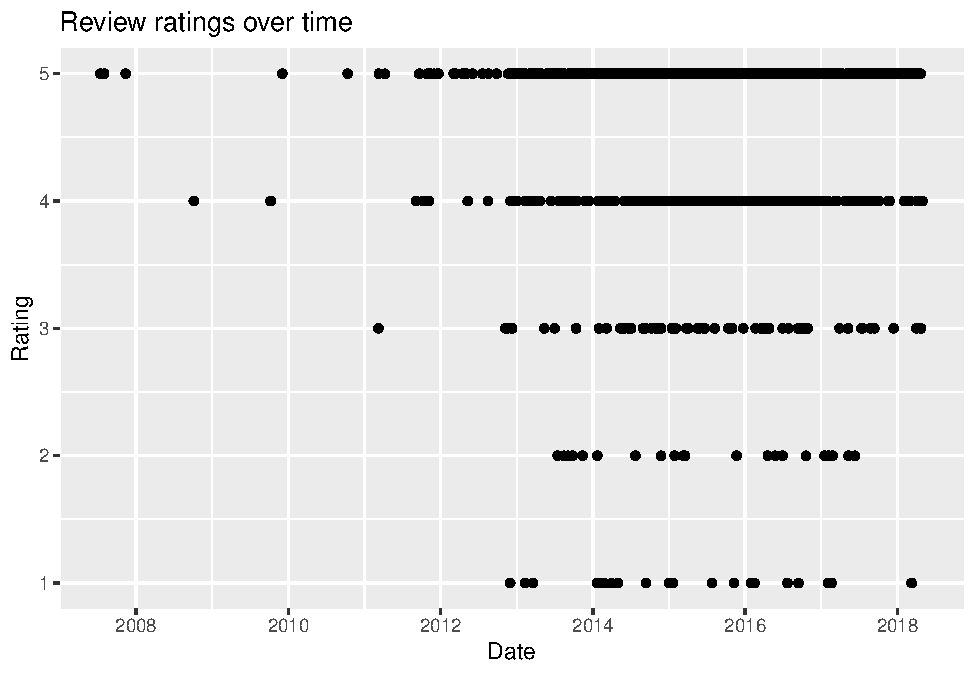
\includegraphics{Assignment-STAT702_files/figure-latex/3a plots-4.pdf}

\hypertarget{question-3b}{%
\subsection{Question 3b}\label{question-3b}}

\hypertarget{using-the-review-text-reviewtext-and-any-other-variables-you-think-are-relevant-investigate-the-customer-sentiment-towards-and-satisfactiondissatisfaction-with-the-product-that-has-been-assigned-to-your-group.-your-answer-should-include-a-word-cloud-and-a-sentiment-analysis.}{%
\subsection{Using the review text (reviewText) and any other variables
you think are relevant, investigate the customer sentiment towards, and
satisfaction/dissatisfaction with, the product that has been assigned to
your group. Your answer should include a word cloud and a sentiment
analysis.}\label{using-the-review-text-reviewtext-and-any-other-variables-you-think-are-relevant-investigate-the-customer-sentiment-towards-and-satisfactiondissatisfaction-with-the-product-that-has-been-assigned-to-your-group.-your-answer-should-include-a-word-cloud-and-a-sentiment-analysis.}}

• Appropriate methods are used to tidy the text data.

• Correctly construct and interpret a word cloud of the reviewText
variable.

• Correctly perform and interpret a sentiment analysis of the reviewText
variable.

• Correctly perform and interpret some additional analysis of the
reviewText variable, incorporating at least one other variable from the
dataset.

• Interpretations of analyses are correct, provide insight and are
written at an appropriate level for a manager.

\hypertarget{answer-3}{%
\subsection{Answer}\label{answer-3}}

Review text has been tokenised and stop words have been removed. Stop
words are words such as `the' and `it' that hold little information for
sentiment analysis. The top 10 words in reviews are plotted below along
with their frequency.

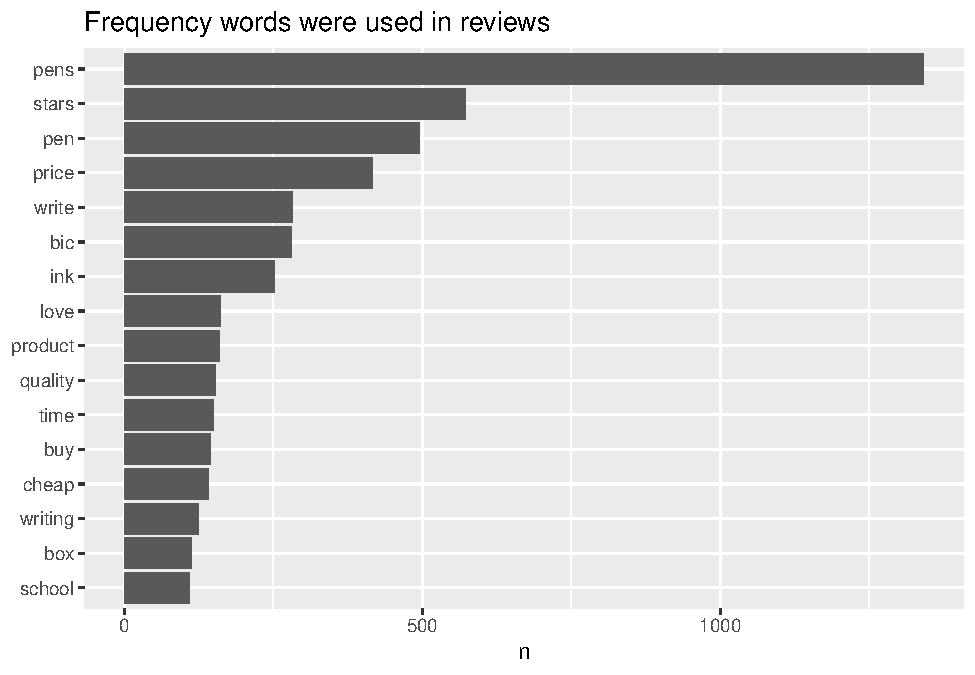
\includegraphics{Assignment-STAT702_files/figure-latex/3b word frequency-1.pdf}

Notably the top words are `pens', `stars' and `pen'. The product that is
being analysed is bic pens, this explains why these words occur
frequently. Users provide a 5 star rating, in their review users then
refer to their rating and this explains why the word `stars' occurs
frequently. These words offer little information about how reviewers
feel about the product so these are removed from reviews for the next
part of analysis.

The remaining words are given a sentiment rating, high ratings indicate
positive sentiment and low ratings indicate negative sentiment. The top
10 frequently used negative and positive words are presented below along
with a word cloud of the top 100 words.

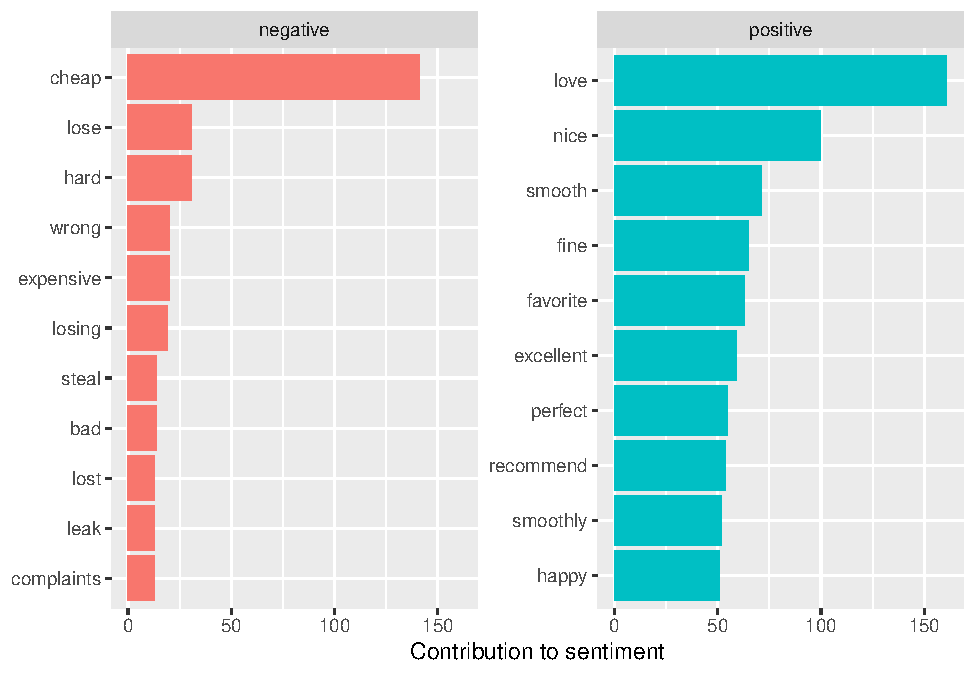
\includegraphics{Assignment-STAT702_files/figure-latex/3b word sentiment-1.pdf}
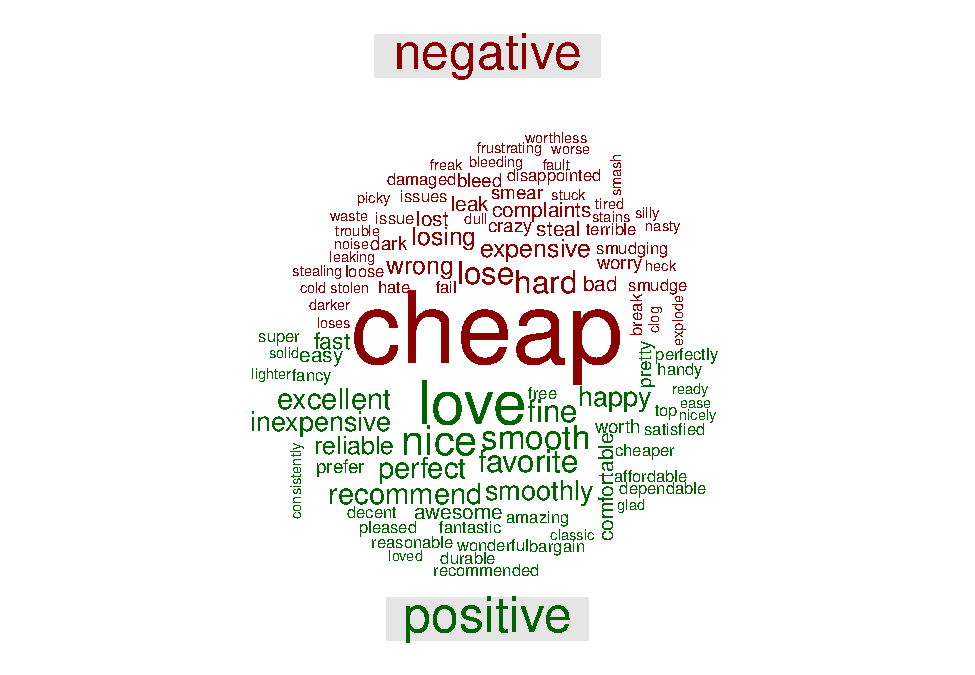
\includegraphics{Assignment-STAT702_files/figure-latex/3b word sentiment-2.pdf}

Notably the word `cheap' is the most commonly used negative word and is
used significantly more frequently than any other negative word. `Cheap'
can be used to say something is low quality, however in the context of a
pen `cheap' is likely to be a positive descriptor as people often don't
want to spend too much money on pens. Overall 141 reviews included the
word `cheap', 0.7446809\% were 5 star reviews and 0.1560284\% were 4
star reviews. This indicates that `cheap' is more likely to indicate a
positive rather than negative sentiment.

For each review the word sentiments are added together giving the review
an overall sentiment score. Below is a plot showing the proportion of
reviews in each rating category were given an overall negative or
positive sentiment rating. When the word `cheap' is excluded there is a
small change with a decreased proportion of 3-5 ratings classified as
negative. This indicates better performance classification.

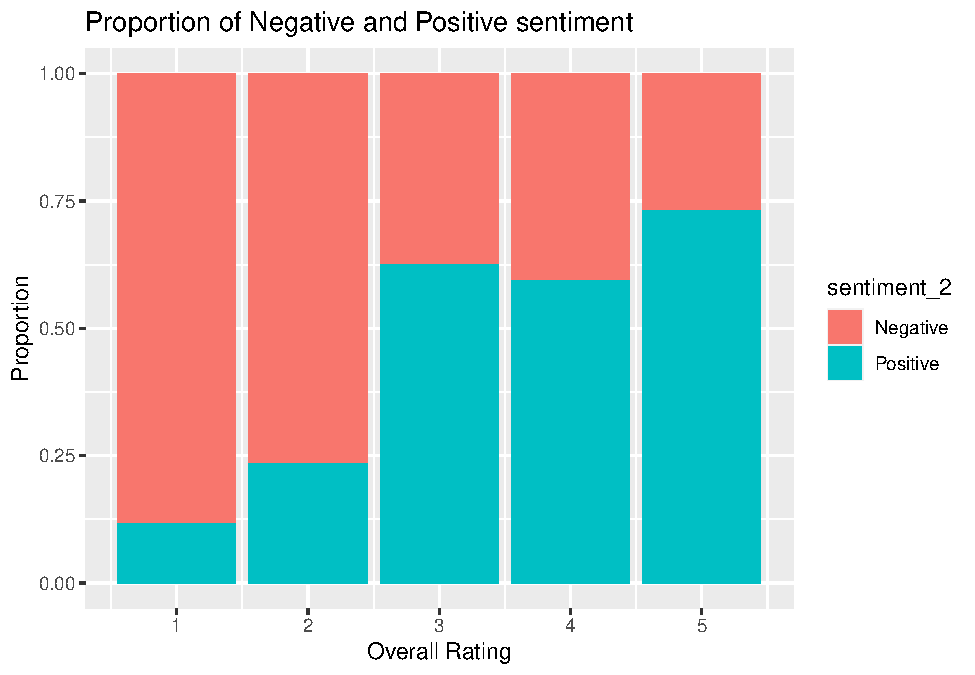
\includegraphics{Assignment-STAT702_files/figure-latex/unnamed-chunk-2-1.pdf}
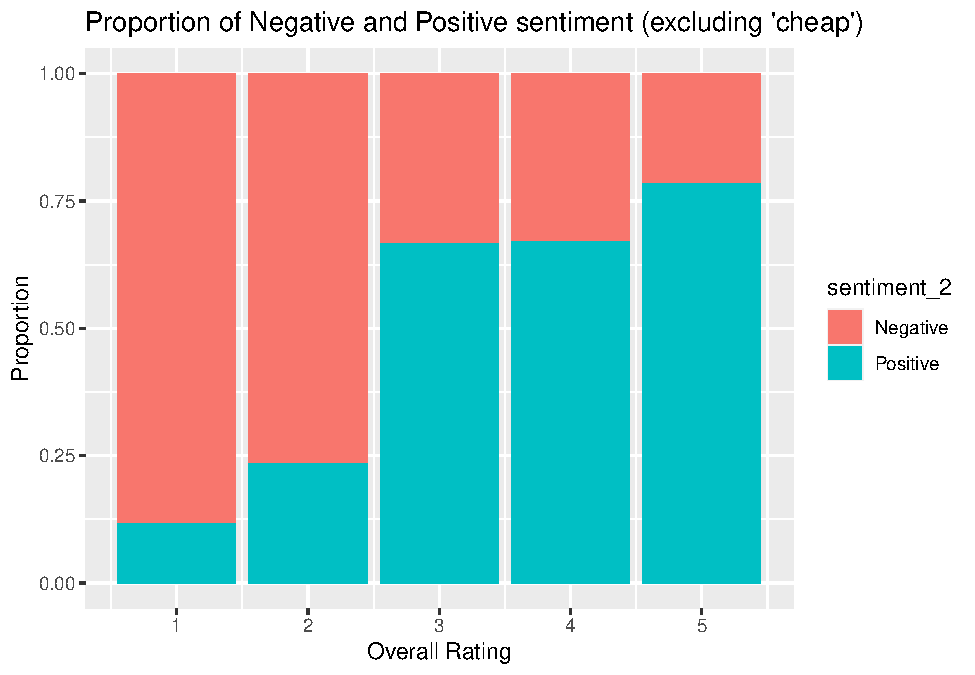
\includegraphics{Assignment-STAT702_files/figure-latex/unnamed-chunk-2-2.pdf}

end
\#\#\#\#\#\#\#\#\#\#\#\#\#\#\#\#\#\#\#\#\#\#\#\#\#\#\#\#\#\#\#\#\#\#\#\#\#\#\#\#\#\#\#\#\#\#\#\#\#\#\#\#\#\#\#\#\#\#\#\#\#\#\#\#\#\#

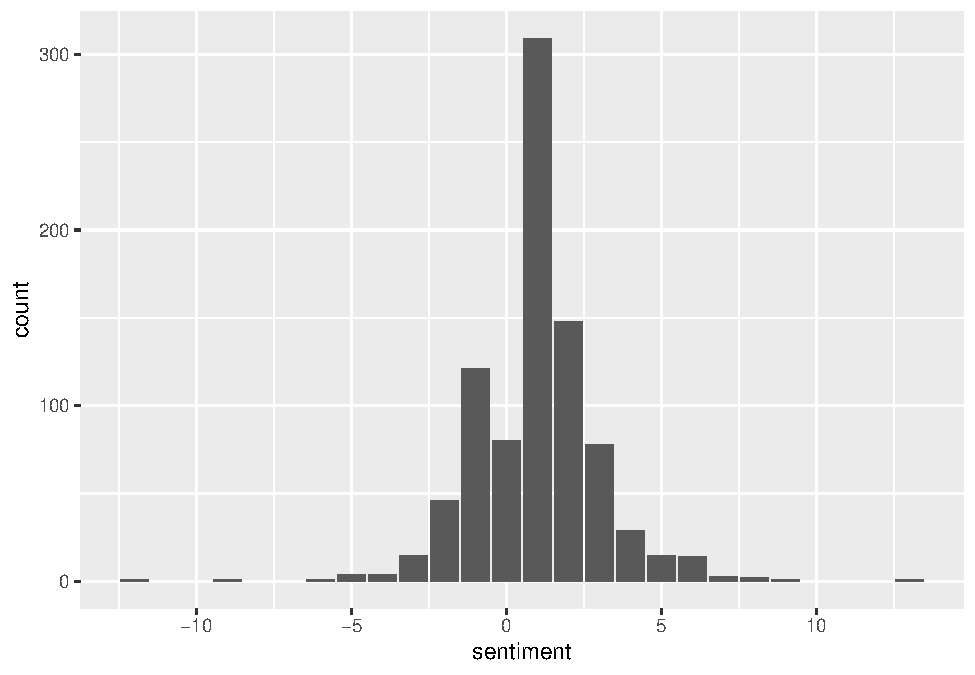
\includegraphics{Assignment-STAT702_files/figure-latex/unnamed-chunk-3-1.pdf}

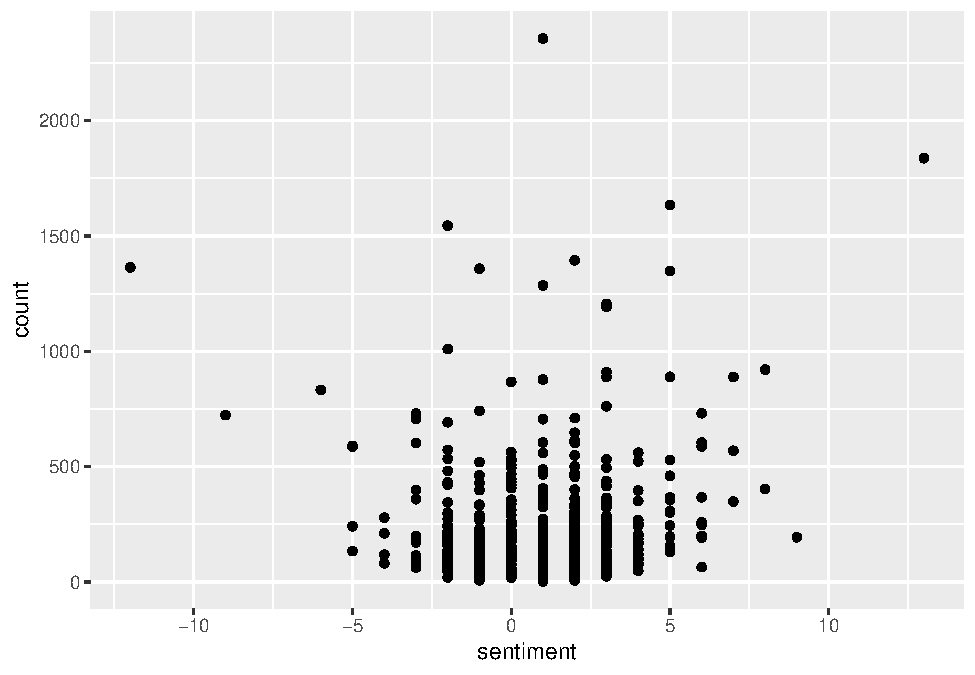
\includegraphics{Assignment-STAT702_files/figure-latex/unnamed-chunk-4-1.pdf}

Using tidytext, going to tidy the data. First, we select the rows we
want to use for the sentiment analysis

\begin{verbatim}
## # A tibble: 6 x 6
##   document.id overall verified reviewText             summary         date      
##         <int>   <int> <lgl>    <chr>                  <chr>           <date>    
## 1       48735       4 TRUE     Good quality bulk pen~ Four Stars      2018-05-01
## 2       48762       3 TRUE     I bought six boxes, f~ five boxes are~ 2018-04-24
## 3       48763       5 TRUE     These pens consistent~ consistently w~ 2018-04-22
## 4       48774       5 TRUE     They're pens. What el~ Cheap Price fo~ 2018-04-21
## 5       48775       5 TRUE     Good Good              Five Stars      2018-04-16
## 6       48776       4 TRUE     Classic pen.  Average~ Good Deal       2018-04-10
\end{verbatim}

We clean the data by using \texttt{unnest\_tokens} to tokenize the
\texttt{reviewText} column. We also add a column representing the line
number for the data

\begin{verbatim}
## # A tibble: 6 x 7
##   document.id overall verified summary    date       reviewWord linenumber
##         <int>   <int> <lgl>    <chr>      <date>     <chr>           <int>
## 1       48735       4 TRUE     Four Stars 2018-05-01 good                1
## 2       48735       4 TRUE     Four Stars 2018-05-01 quality             2
## 3       48735       4 TRUE     Four Stars 2018-05-01 bulk                3
## 4       48735       4 TRUE     Four Stars 2018-05-01 pens                4
## 5       48735       4 TRUE     Four Stars 2018-05-01 especially          5
## 6       48735       4 TRUE     Four Stars 2018-05-01 for                 6
\end{verbatim}

Now, we remove the stop words. Our stop words are taken from the
\texttt{stop\_words} dataset included in tidytext. By using an
anti\_join, we are able to filter out the stop words.

Below, we plot the words in the cleaned dataset, according to the number
of times they are present in the dataset.
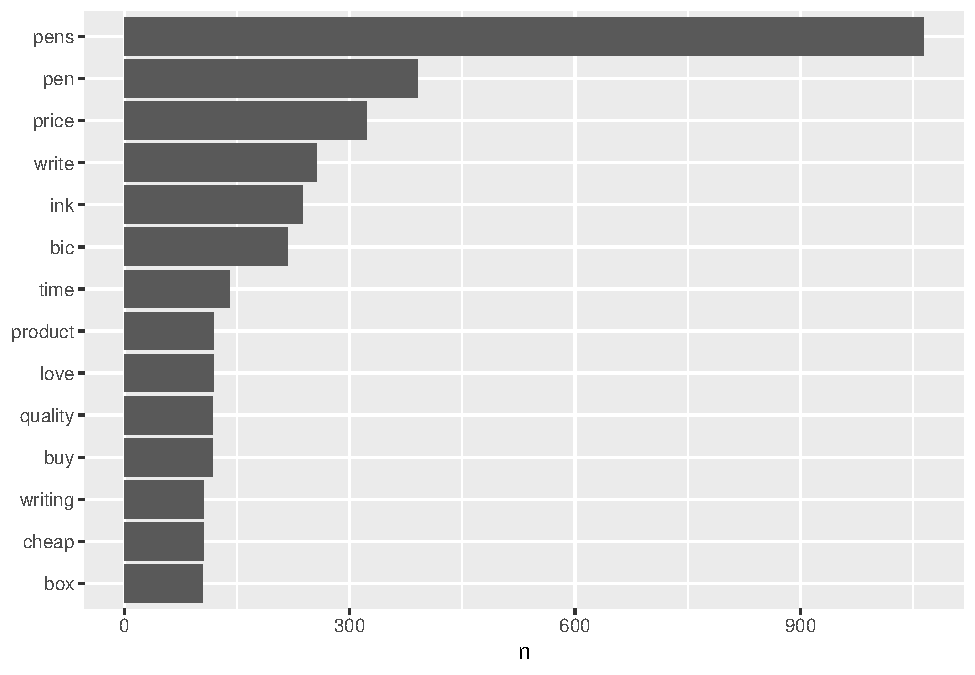
\includegraphics{Assignment-STAT702_files/figure-latex/preliminary analysis-1.pdf}
On an initial analysis, we can see that the word \texttt{pen(s)} has
been used the most. Since this word describes our product, it is used
quite often in the reviews. After that, customers mention the price of
the item a lot more than any thing else. The rest of the words are used
to describe the product and it's features.

Using the

\begin{verbatim}
## # A tibble: 6 x 6
##   document.id overall negative positive sentiment linenumber
##         <int>   <int>    <dbl>    <dbl>     <dbl>      <int>
## 1       48762       3        1        0        -1          1
## 2       48763       5        0        1         1          2
## 3       48774       5        0        2         2          3
## 4       48776       4        0        1         1          4
## 5       48803       5        0        2         2          5
## 6       48837       5        1        2         1          6
\end{verbatim}

The mean sentiment of all reviews is 0.7593261.

We plot the
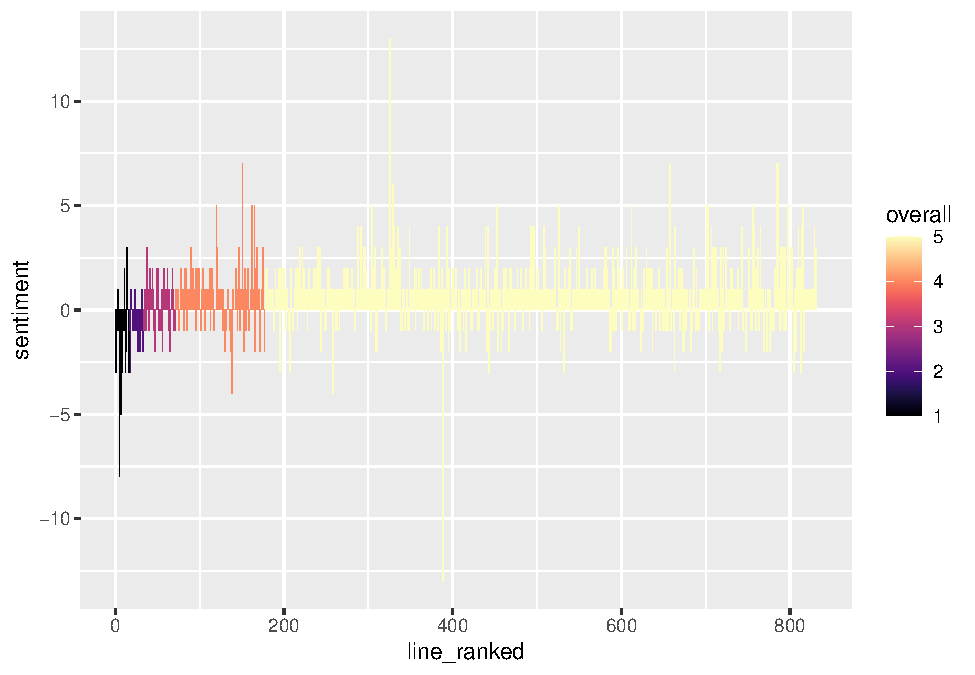
\includegraphics{Assignment-STAT702_files/figure-latex/sentiment_plot-1.pdf}
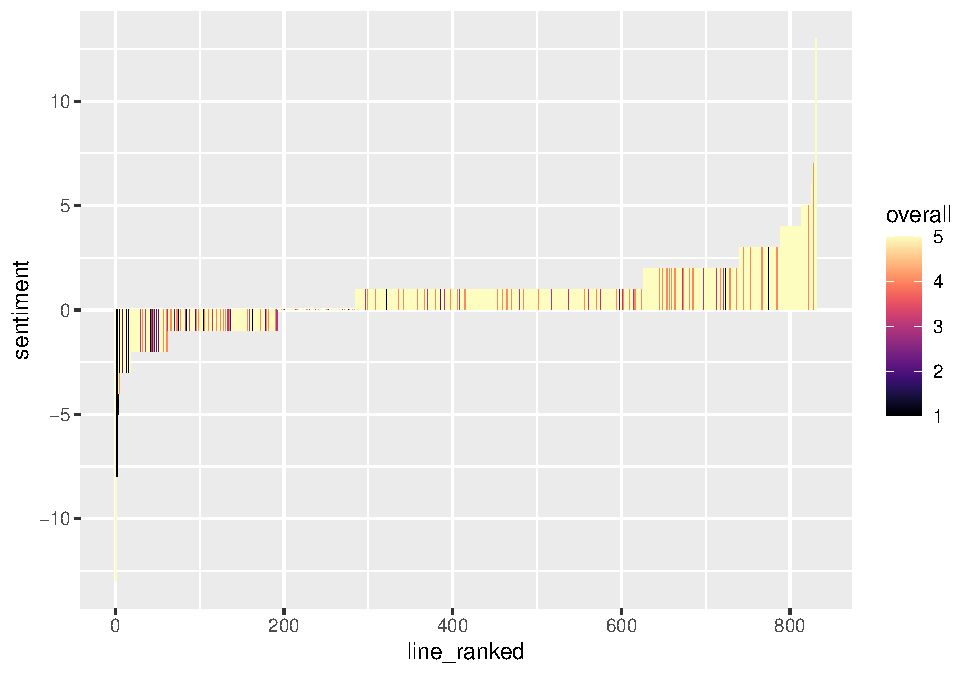
\includegraphics{Assignment-STAT702_files/figure-latex/sentiment_plot-2.pdf}
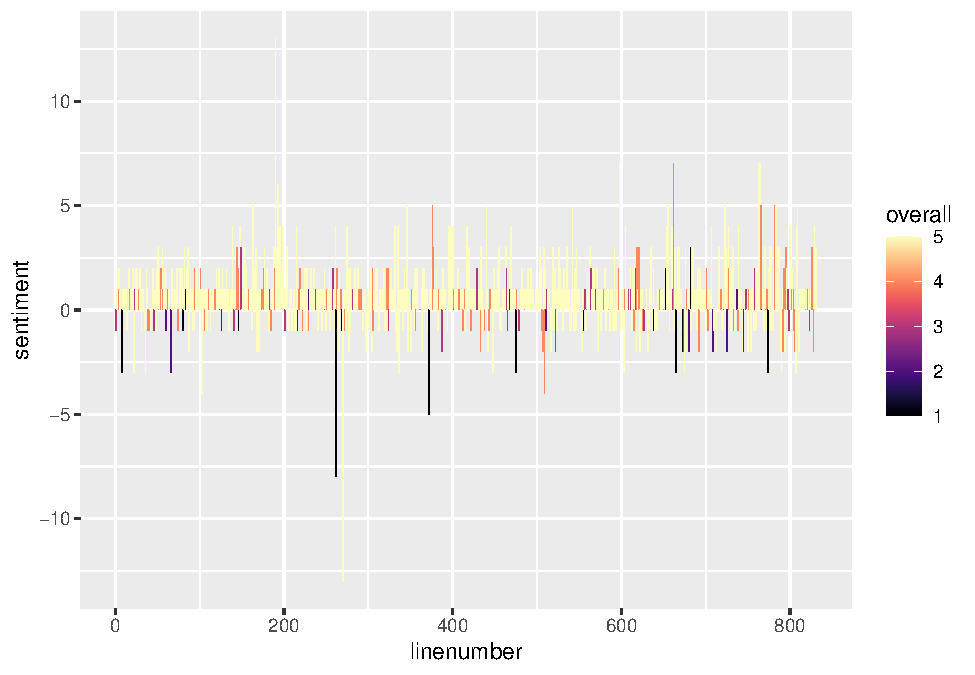
\includegraphics{Assignment-STAT702_files/figure-latex/sentiment_plot-3.pdf}
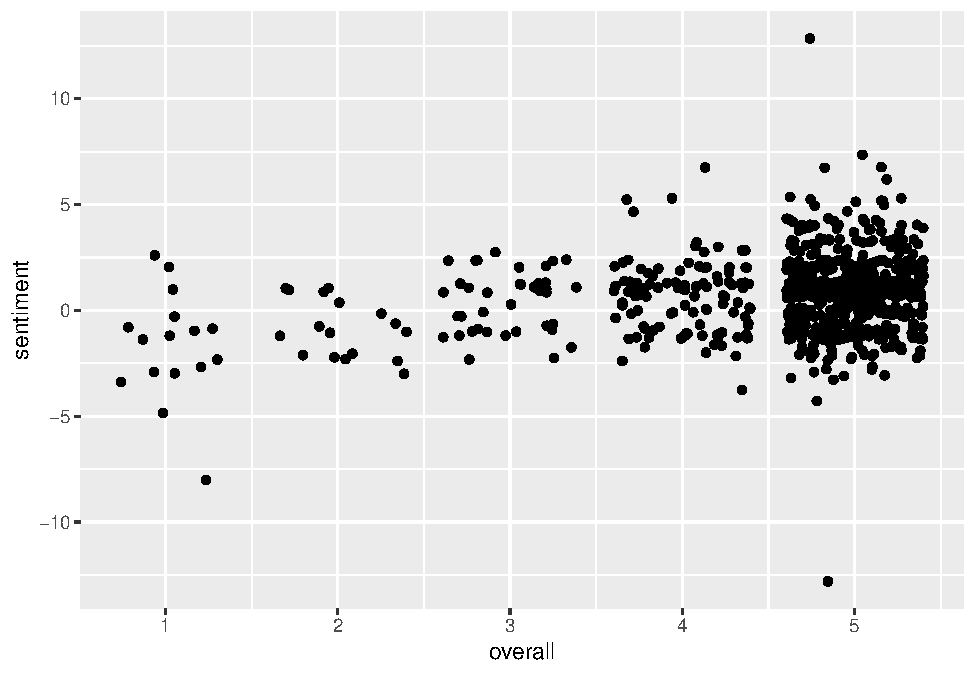
\includegraphics{Assignment-STAT702_files/figure-latex/sentiment_plot-4.pdf}
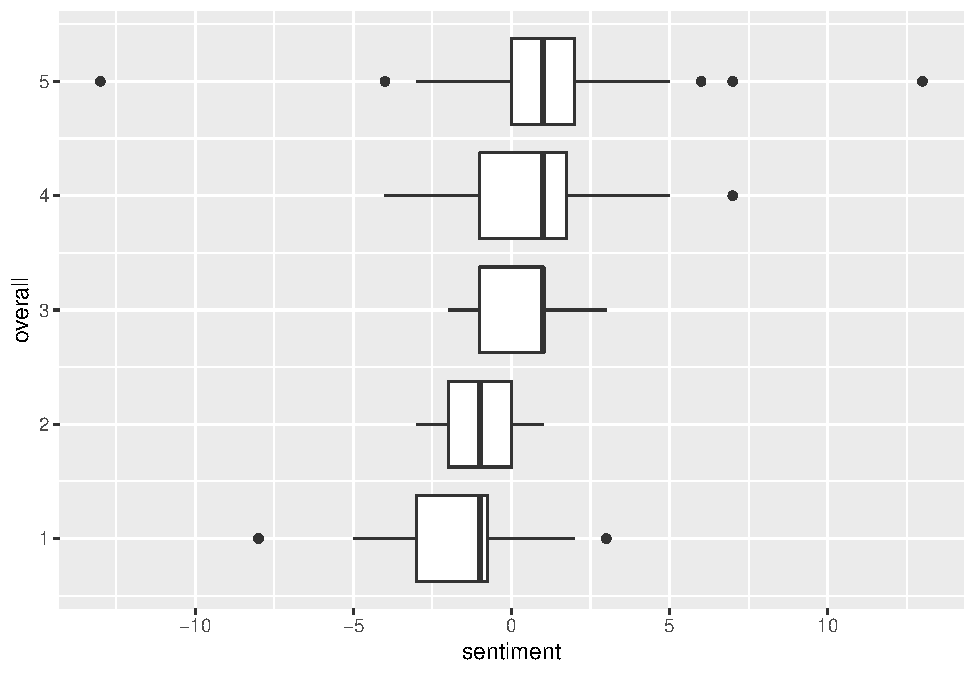
\includegraphics{Assignment-STAT702_files/figure-latex/sentiment_plot-5.pdf}

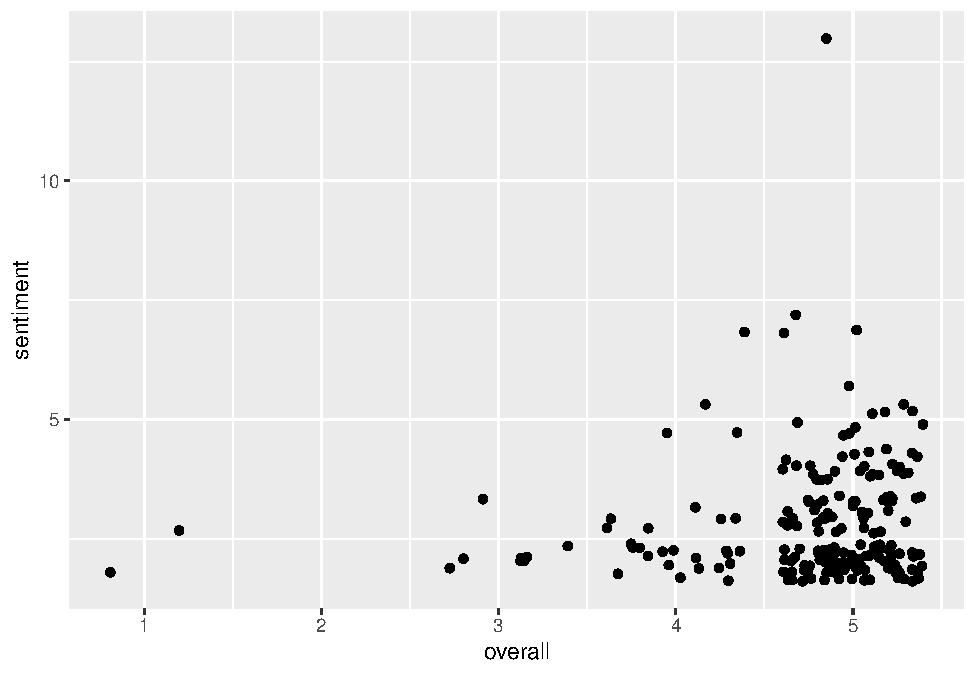
\includegraphics{Assignment-STAT702_files/figure-latex/top100_positive-1.pdf}

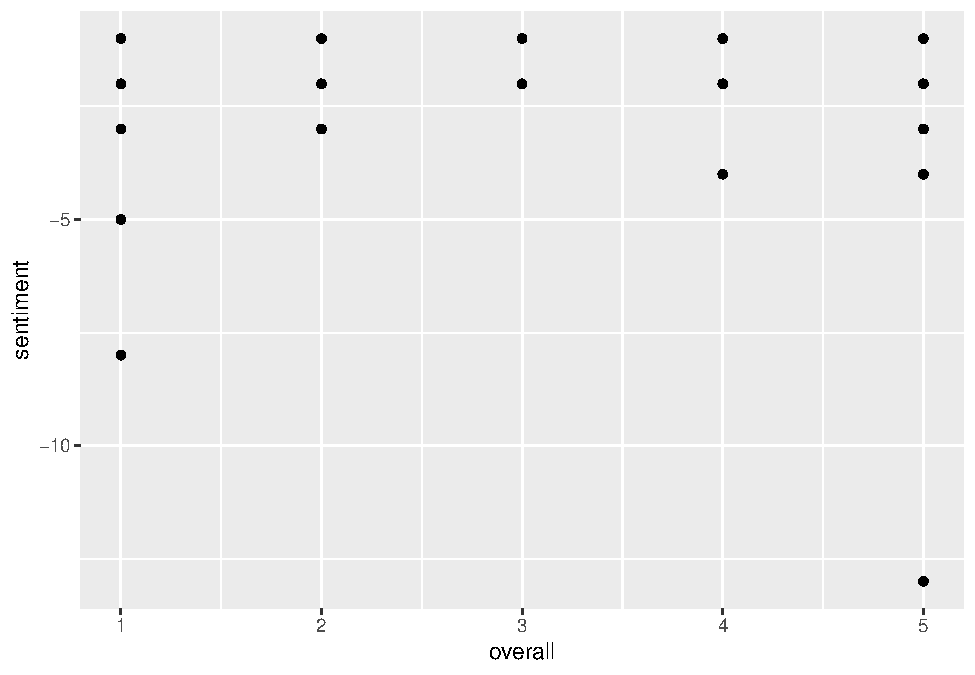
\includegraphics{Assignment-STAT702_files/figure-latex/top100_negative-1.pdf}

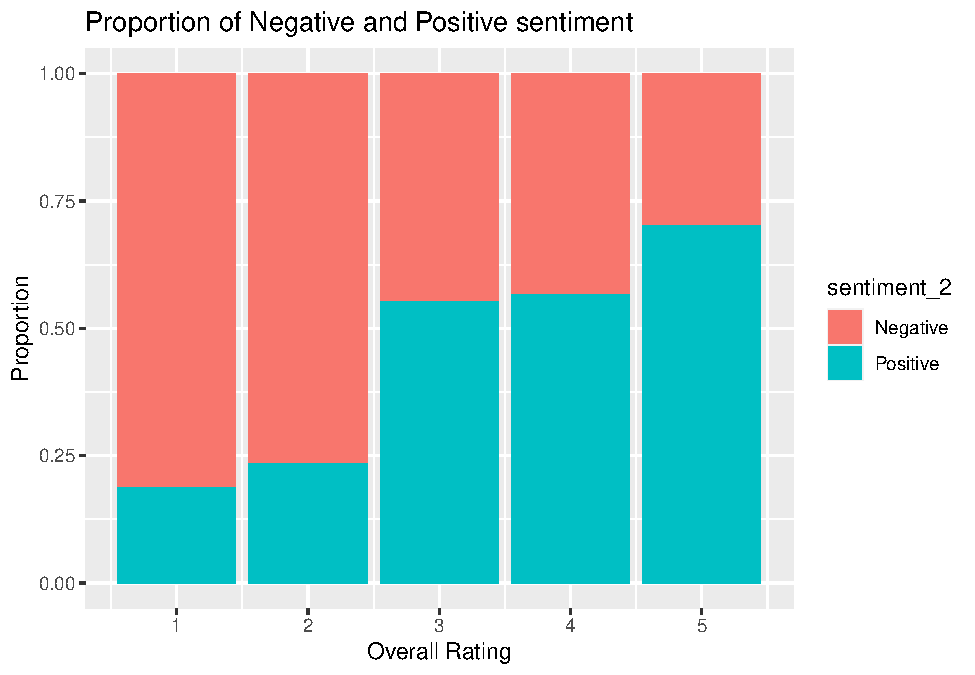
\includegraphics{Assignment-STAT702_files/figure-latex/proportion-1.pdf}

Finally, we plot the words against their occurance, based on their
contributions to the sentiment.
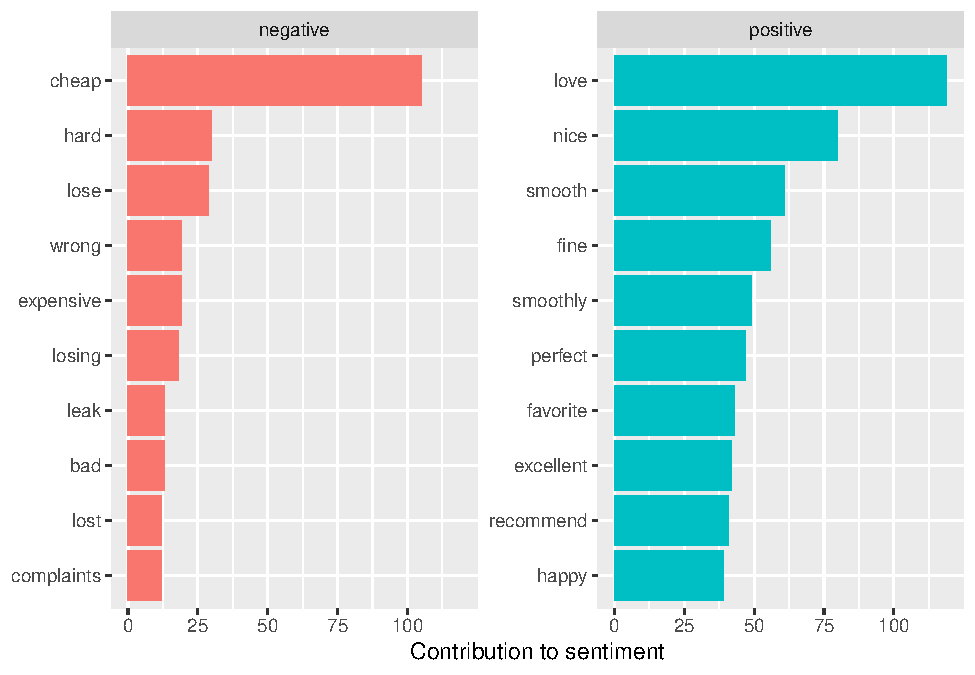
\includegraphics{Assignment-STAT702_files/figure-latex/plot_by_sentiment-1.pdf}
The word \texttt{cheap} contributes the most to negative reviews and the
word \texttt{love} contributes most to the positive reviews.

Conducting the analysis, one can safely say that the price and user's
experience contribute greatly to the sentiment of a customer's review.
If a customer's purchase contains itms that tend to be defective, their
review is going to be more negative.

On the other hand, most of the reviews are positive, with a rating
between four and five stars. The words in the convetributing to a
positive sentiment depict a positive user experience. The user also
tends to recommend the product to other potential users if they have a
positive experience.

\end{document}
